% !Mode:: "TeX:UTF-8"
\documentclass[master,openright,twoside,color]{buaathesis}
\usepackage{epsfig,endnotes}
\usepackage{color}
\usepackage{amssymb}
\usepackage{algorithm}
\usepackage{algorithmic}
\usepackage{graphicx,subfigure}
\DeclareGraphicsExtensions{.eps,.ps,.eps.gz,.ps.gz,.eps.Z}
\usepackage{stfloats}
\usepackage{float}
\usepackage{caption}
\usepackage{multirow}

\begin{document}

% 用户信息
% !Mode:: "TeX:UTF-8"

% 学院中英文名,中文不需要“学院”二字
% 院系英文名可从以下导航页面进入各个学院的主页查看
% http://www.buaa.edu.cn/xyykc/index.htm
\school
{软件学院}{School of Software}

% 专业中英文名
\major
{软件工程与管理}{Software Engineering and Management}

% 论文中英文标题
\thesistitle
{基于海量交通数据挖掘的出租移动模型的研究与实现}
{ }
{How to design the BUAA-thesis with \LaTeX{} very very very very very very long}
{ }
% 作者中英文名
\thesisauthor
{杨文静}{Wenjing Yang}

% 导师中英文名
\teacher
{王海泉}{Haiquan Wang}
% 副导师中英文名
% 注:慎用‘副导师’,见北航研究生毕业论文规范
%\subteacher{副导师}{subteacher}

% 中图分类号,可在 http://www.ztflh.com/ 查询
\category{TP312}

% 本科生为毕设开始时间;研究生为学习开始时间
\thesisbegin{2011}{09}{01}

% 本科生为毕设结束时间;研究生为学习结束时间
\thesisend{2012}{07}{01}

% 毕设答辩时间
\defense{2012}{06}{01}

% 中文摘要关键字
\ckeyword{车辆移动模型,海量数据,}

% 英文摘要关键字
\ekeyword{BHOSC, \LaTeX{}, Thesis}

% !Mode:: "TeX:UTF-8"

% 研究方向
\direction{车辆移动模型}

% 导师职称中英文
\teacherdegree{教授}{Prof.}
% 副导师职称中英文
% 注:慎用‘副导师’,见北航研究生毕业论文规范
%\subteacherdegree{讲师}{Teacher}

% 保密等级,注:非保密论文时不需要此项
%保密论文请更改‘buaathesis.cls’里相应代码
%\mibao{机密}

%申请学位级别
\applydegree{全日制工程硕士}

% 论文编号,由10006+学号组成
\thesisID{10006SY0000000}

% 论文提交时间
\commit{2012}{03}{03}

% 学位授予日期
\award{2012}{04}{04}


% 中英封面、提名页、授权书
\maketitle
% 前言页眉页脚样式
\pagestyle{frontmatter}
% 摘要
% !Mode:: "TeX:UTF-8"

% 中英文摘要
\begin{cabstract}
在交通领域中,交通瓶颈的预测以及寻径算法的验证大都建立在仿真环境中。类似的,车联网中路由协议的验证也是建立在仿真平台上。而其中的难点在于如果提高仿真的准确性。移动模型是现有的车辆仿真的基础,对提高仿真的准确性具有重要意义。基于海量交通数据挖掘的出租移动模型是基于北京市12000多辆出租车的移动轨迹进行分析建模。首先由日常观察和经验出发,提出假设,假设出租车的移动行为与出租车载客和空载状态,时间以及车辆地理位置有关。然后分别从车辆状态,时间和地理位置角度分析北京市的出租车数据,分析结果证明我们提出的三个假设合理。然后对北京市出租车从宏观和微观角度建模。宏观角度,我们按照时间和载客/下客事件划分区域并基于海量交通数据分别计算载客区域到下客区域以及下客区域到载客区域的转移概率矩阵。微观方面,抽取北京市地图,定义寻径算法以及对车辆速度建模。由于我们考虑到了车辆的状态和时间因素,区域划分和区域转移概率矩阵会随时间和状态的变化而相应变化。在实验验证方面,我们验证了车辆的接触指标以及车辆的出入度指标,并与实际数据,随机路点移动模型最短路径移动模型相比较。实验证明相对于其他移动模型,基于海量交通数据的移动模型和实际数据的接触特征最为相似。出入度方面,每天的实际轨迹出入度与平均实际轨迹区域出入度的相对误差仅为$10\%$,本文提出的移动模型与实际轨迹平均区域出入度的相对误差为$47\%-49\%$,而其他移动模型的相对误差达到$65\%-69\%$和$81\%-83\%$,准确性提高了$10\%-40\%$.实验结果表明本文提出的移动模型具有较高的仿真相似性。

\end{cabstract}

\begin{eabstract}
The mobility model is one of the most important factors that impacts the evaluation of any transportation vehicular networking protocols via simulations. However, to obtain a realistic mobility model in the dynamic urban environment is very challenging. Recently, several studies extract mobility models from large-scale real data sets (mostly taxi GPS data) without consideration of the statuses of taxi. In this paper, we discover three simple observations related to the taxi statuses via mining of real taxi traces: (1) the behavior of taxi will be influenced by the statuses, (2) the macroscopic movement is related with different geographic features in corresponding status, and (3) the taxi load/drop events are varied with time. 
Based on these three observations, a novel taxi mobility model (T-START) is proposed with respect to taxi statuses, geographic region and time. The simulation results illustrate that proposed mobility model has a good approximation with reality in trace samples and distribution of nodes in four typical time period.
\end{eabstract}
% 目录、插图目录、表格目录
\tableofcontents
\listoffigures
\listoftables
% 符号表
\include{data/master/denotation}

% 正文页码样式
\mainmatter
% 正文页眉页脚样式
\pagestyle{mainmatter}

% 正文
% !Mode:: "TeX:UTF-8"
\chapter{绪论}

本章首先介绍背景与意义,结合车联网以及交通领域的应用背景指出论文的研究意义与价值,并给出课题来源的介绍。其次,结合国内外研究现状,探究了现有的移动模型研究,并分析了其中存在的问题。然后针对这些问题提出了本文的研究目标,思路与研究内容。最后就论文的组织与安排进行了必要的介绍与说明。

\section{研究背景与意义}
<智能交通技术的发展现状>

本课题来源是国家自然科学基金(No. 61170295)项目, 该项目旨在发现出租车行为模式,为智能交通系统提供更为完善的理论支持。
\section{国内外研究现状}
本章主要对国内外移动模型现状进行综述,针对移动模型的约束信息和依赖信息,从随机移动模型、概率约束移动模型、节点关系依赖的移动模型、地理受限移动模型、基于真实地图的移动模型、引入交通特征的移动模型和基于真实轨迹的移动模型几方面进行综述。
\subsection{随机移动模型}

随机移动模型是指节点运动方向速度随机的移动模型。由于其模型简单,依赖信息少可以简单描述节点移动,被广泛应用到基于移动模型的仿真研究中。

随机游走模型(Random walk mobility model, RW)[5]是由Einstein提出的用于模拟物理粒子的布朗运动。节点在每段独立时间t内,随机选择移动方向和移动速度,当到达边界时,遵循反射定律按照一定角度反弹后回到场景中继续移动。随机游走模型在仿真中经常被用于模拟人类在无障碍的场景中的移动行为。

随机路点模型(Random Waypoint model, RWP)[6]与RW的不同之处在于不是固定时间,而是在一段路径开始时,随机选取下一步的目标点,并随机生成速度。到达目的点后,会定义一个暂停时间,暂停时间也是从一个范围内随机生成的。因此在随机路点模型中不用考虑边界问题。随机路点模型被广泛用于车载网络的仿真中。随机路点移动模型节点都在初始位置周围运动,但是节点可能无法遍布仿真区域,节点分布不均匀。

随机方向模型(Random Direction model, RD)[7]被应用与多种自组网协议中。它定义节点运动为匀速,节点方向从[0,2ᴨ]角度内均匀选择一个方向,直到运动到区域边界点D。然后保持静止时间t, 然后以此点为初始节点,重复以上运动[1]。但是RD模型在空间分布上表现出不均匀的特质,中心概率密度小,边界概率密度大。

以上三种模型是经典的移动模型,在移动方式方面没有利用任何先验知识,适用于简化的移动场景中。

\subsection{概率约束的移动模型}
    基于概率矩阵的随机漫步模型(Probabilistic version of random walk mobility model)[2]采用三个状态来决定移动方向,1是开始位置,0是之前的位置,2是下一步的位置。通过三个状态的转移矩阵来确定下一步的方向。
2002年,Hsu等人提出了加权路径点模型(Weighted Way Point model)[8]。该模型对较高访问频率的热点区域,目的地的选择与当前时间和位置有关,每个位置有不同的暂停时间。
	
	高斯-马尔科夫模型(Gauss-Markov model)[9]采用马尔科夫链模型,认为第n次的运动与前一次运动的速度、方向等有关。其速度和方向是符合高斯分布的随机变量。

2001年,Bettstetter等人[10]提出平滑随机移动模型(Smooth Random Mobility model),该模型是在RD基础上的改进。节点的速率和方向是和时间相关的使得模型速率和方向上的改变时平滑的。速率控制的思想是设定一个目标速率,使得加速度线性变化,最后达到目标速率。这个过程符合泊松分布。节点的方向变化与速率相关,节点速率小轨迹的半径小,速度偏转大,反之,节点速度大时,轨迹的半径也随之变大。

\subsection{节点相互依赖的移动模型}
2004年,Musolesi, M.等[11]提出了基于社会关系的移动模型。采用加权图表示社会关系网络,权值用来衡量个体之间交互关系的强弱。每个节点都具有社交因子(Social Factor, SF)用来衡量与其他节点的态度。

另一类移动模型中节点以组的形式移动。队列移动模型(Column Mobility Model)[12]定义一组节点以统一方向移动。追逐移动模型(pursue mobility model)模拟节点追逐某物时的移动模式,按照加速函数来确定节点的速度。游牧团体移动模型
(Nomadic Community Mobility Model)定义一组节点共同从一个区域移动到另一个区域的运动模式。通过定义参考点,组内节点在参考点附近随机移动。当参考点运动时,组内节点会向参考点附近游走。

\subsection{地理受限制的移动模型}

  1) 人为规定的地理受限移动模型

曼哈顿模型(Manhattan mobility model)[13]是通过对曼哈顿街区建模,并规定节点按照街道模型移动的移动模型。节点在城区地图中沿着垂直或水平的方向移动。在十字路口节点可以选择直行,或者转向。类似的移动模型有市区移动模型[14]。该模型将对街道的建模精细化,由简单的网格街道变为模拟市区内的公路或街道的移动模型。文献[15]结合了交通理论,将地理信息分为市区、地区和街区,并依据此建模。另一类移动模型,关注在地理上的限制区域。文献[16]对建筑物等障碍物建模,提出了障碍物移动模型。
 
 2)基于真实地图的移动模型
 
 1999年,Hong, X.[17]等人提出了Reference Point Group Mobility (RPGM)用于表现移动主机的关系。实验验证了移动模型对网络协议和性能的影响,验证了移动性对分簇和网络性能的影响。研究发现移动性增加,连接变化更为频繁,移动性增加,簇头变化更为频繁,移动性增加,负载变化。RPGM也是一种群主移动模型。

2004年,Bhattacharjee, D.等人提出了混合移动模型[18]。该模型在加州大学圣迭戈分校校园内采集AP数据,收集用户轨迹,并通过统计分析来建立模型,可以用来预测节点的位置。

2004年,Saha, A.K[19]等引入了实际道路,对车载网络建模。实验验证从路由性能等方面与RWP模型进行了比较,发现两者的不同。

2005年,Jain R等人[20]采用Dartmouth 大学校园收集的真实的轨迹数据

2005年,文献[21]提出了车载无线网络综合模型和交通模型。该模型基于由真实路网简化的道路模型来验证ad hoc网络性能。提出了基于道路的移动模型STRAW. 验证发现该模型的网络性能与RWP模型差别非常大。此外,文献还验证了不同城市环境中的网络性能,发现节点增多的时候芝加哥和波士顿的场景中平均速度会减小,和投递率。该模型基于真实的道路信息,验证了RWP模型无法表现出城市车载网络的特征。

这些移动模型探究在加入了地理信息后,移动模型在网络性能、移动特征等方面的影响,在验证方面没有与真实的数据比较,因此难以说明模型的真实性。
 
4)引入交通特征的移动模型

从对车流的刻画粒度上,可以将移动模型分为宏观、微观和宏观微观结合的移动模型。宏观模型将车流看作连续流体,忽略车辆的细节行为。微观模型则对节点行为进行细粒度的刻画。关注节点速率、方向、加速度、交通灯情况等。但是一个真实的移动模型需要同时考虑车辆宏观和微观的特征。车辆移动模型需要关注车辆密度、车流等宏观特征,也需要考察车辆的间距、加速度、刹车、超车等微观特征。

1992年,Seskar, Ivan等人在文献[22]中讨论了移动网络中轨迹跟踪的问题,并基于真实的交通参数的关系建立了车辆移动模型(Fluid Traffic Model,FTM)。该模型给出了车辆速度与车流密度之间的关系,即当车流密度增加时,车辆速度会相应地减慢, 并在实验验证中观察了该模型的适用场景。

2000年,Treiber, M.从德国高速公路采集到的数据中发现,几种不同类型的拥塞发生在不同的地段,分别是关闭通道的道路、十字路口和上坡路等,并分析了各种不同拥塞以及混合型拥塞发生的状况,在文献[23]中提出智能驾驶员模型(Intelligent Driver Model,IDM),它是一个连续的微观单通道模型,将相邻车辆行为进行关联,建立车辆跟随模型,实验结果表明,该模型可以用来发现图瓶颈的更通用方式。VanetMobiSim[24]优化了 IDM 模型,引入了对十字路口和多车道的控制,设计了具有十字路口管理的移动模型(Intelligent  Driving  Model  with Intersection Management,IDM-IM)和可切换车道的移动模型(Intelligent Driving Model with Lane Change,IDM-LC)。

2011年,Helbing, D等人[25]对“幻像交通拥塞”、走走停停(stop-and-go)交通现象的产生机制、不同拥塞的产生原因和相关之处、当将要达到道路交通能力时交通堵塞最为严重、暂时减少交通量是否会造成交通堵塞等现象和问题进行了解释,并依据此为自动(self-driven)多组分(many-particle)系统建立了一个通用的模型框架。
引入交通特征的移动模型,对车辆间的关系以及关系对车辆微观行为的影响较为关注。文献[23]等研究者同时也引入了交通数据,用于研究真实场景中的拥塞分类和发生的时间和地点。但是关于交通特征的研究过于偏向微观,对宏观现象的解释和建模较为缺乏。

5) 基于实际轨迹的移动模型

2006年,文献[26]采用移动用户数据,对无线网络中的移动节点建模。他们从实际收集的13个月的轨迹数据中发现节点的速度和暂停时间符合对数正太分布,并且节点的运动方向收到道路方向的影响。在此基础上,他们提出了关注热点区域的移动模型。模型的平均相对误差为17%.

2007年,Zhang, X等人提出了基于公交车容断络移动模型[27]。该模型采用UMass DieselNet数据集,该数据集由安装了WiFi设备的公交车组成网络收集而来。通过对数据的研究发现节点对级别的接触并没有明显的规律,然而在路由级别的节点对接触表现出明显规律。基于此发现,他们提出了接触间隔时间生产模型。实验证明基于路由级别的接触生产模型能更准确符合实际路由性能。

同年,Hsu, W等人提出了随时间变化的用户移动模型[28]。该模型采用WLAN轨迹数据。他们利用不均匀的访问地点偏好将社区定义为经常被节点访问的地区,并采用不同参数的时间段来发现在某区域周期性出现的节点。实验结果显示其在hitting time和meeting time两个指标上与实际的相对误差不高于20%.

2010年,Hongyu等人[29]提出基于上海市出租车GPS数据的城市移动模型。该模型分为宏观和微观两个方面,宏观方面,他们对区域进行了划分,探究区域间的转移概率。微观方面,他们对车辆速度和运行方向进行建模。该模型中引入了城市路网,因此在出租车方向的选择方面,他们对路口的转向进行了建模。验证结果表明,该模型与实际具有很好的相似性。
由于数据集难以获取,并且难以达到统一,因此现有的研究者从真实数据集出发建立的模型较少,模型验证也偏向于说明模型是否达到预期的指标,仿真现象是否符合常识推断,难以与真实数据集相比较。基于大规模真实数据集的移动模型由于数据的准确性、难获取性建模较为困难。在出租车数据集上建立的移动模型更为少见,文献[29]中建立的模型忽略了出租车在空车和重车时的不同点,会影响移动模型的真实性。

通过分类比较现有的移动模型,我们发现1)经典的随机移动模型和基于概率的随机移动模型具有简单、易于构造和使用的特点,但是由于过于简化并且是依据人们经验得出的,因此不太符合真实的移动场景。在车载网络中情况更为复杂,与道路车辆间的影响都十分相关,因此用此类移动模型进行仿真必然会造成实验结果上的误差。2)地理受限的移动模型考虑到节点运动与道路、地区的相关性,但是对车辆自身具有的主观性等考虑较少。3)引入交通特征的移动模型,比较关注车辆微观行为、交通灯影响、车辆拥塞等情况,对宏观情况的研究比较缺乏。4)基于真实轨迹的移动模型从真实数据的统计结果中发现车辆行为规律,反过来建立模型会较为符合真实情况。但是数据难以获取,使得此类模型较少。

\section{有待解决的问题}

移动模型决定节点如何移动[1, 2]。车辆的移动模式对车辆自组织网络等以车辆为节点的网络的拓扑有直接影响。因此,在基于移动模型的仿真研究中,移动模型是否符合假设的场景对网络性能的评估影响巨大[3]。对车辆移动模型的研究可以提高仿真的有效性,同时发现车辆移动的规律,帮助提高车辆的运行效率,安全性以及网络通信的效率[4]。

基于以上现状,可以发现已有很多研究者从移动模式定义、限制条件、依赖条件等方面对移动模型进行研究。然而针对车辆移动模型,当前研究还存在以下问题:
\begin{itemize}
  \item 
现有移动模型缺乏真实大量的交通数据支持。由于海量交通数据难以获取,并且噪音数据多等原因,现有的移动模型缺乏真实的大规模的数据支持,少有移动模型是从统计规律出发,建立移动模型。
\item 现有移动模型验证缺乏与真实交通数据的对比和与其他移动模型的对比。由于移动模型具有对场景有很强的依赖性,移动模型之间很难横向比对。同时,由于缺乏真实的实验平台和真实的数据支持,车辆移动模型难以验证其有效性。
\item



现有的移动模型缺乏大规模的交通数据支持, 同时现有的移动模型缺乏对出租车行为的特殊性的研究。出租车具有载客和空车两种车辆状态,由经验推断,这两种状态下,出租车的行为也会不同。现有移动模型中有针对公交车的周期性行为建模的,然后由于出租车的随机性大,周期性不明显,使得现有的研究仅笼统的从车辆的速度等方面对出租车行为进行探究,缺少对出租车载客、空车等状态下不同的行为特征的研究。
\end{itemize}



\section{研究目标与内容}

\subsection{论文的研究目标}
本文的主要研究目标有:

   \textbf{发现海量交通数据中的出租车移动特征。}包括车辆移动特性与时间、空间以及自身状态的关系。本文从实际数据出发,观察车辆轨迹随时间,空间的变化情况。分析了车辆速度,持续时长等指标随时间,空间,车辆状态变化是否存在规律性。基于这些分析,建立移动模型。
   
   \textbf{建立移动模型.}宏观方面,建立区域转移矩阵,规定车辆从当前区域到其他区域的移动概率分布。最简单的区域定义是将场景划分成规则的四边形,我们认为这样不能体现出不同区域在出租车在地理上的不同点。
因此,我们将区域划分为细粒度的网格,对相邻的具有相似上客(下客)量的网格聚类为区域。
微观方面,抽象实际地图,实现基于地图的最短路径寻径算法。从实际数据中分时间段获得速度分布,拟合获得对应时段的速度分布函数,产生节点运动速度。因为速度字段是GPS采样数据,不准确,为了减小误差,我们采用一段重车(空车)距离除以时间的方法获取速度,然后研究其速度的分布情况。
基于ONE (Opportunity network environment )仿真平台,实现移动模型。

  \textbf{验证模型的有效性.}
通过文献阅读,我们选取了两个角度的指标,分别是出入度和接触指标。以此来验证模型是否具有较强的真实性。


根据以上研究目标,本文的研究内容也可以分为以下三部分。
\begin{itemize}
  \item 发现海量交通数据中的出租车移动特征:
  \begin{itemize}
  \item 宏观统计出租车整体的速度、各个状态的速度、状态持续时间等。
  \item 统计各个时段出租车的分布情况,以及载客、下客事件的分布情况。
  \end{itemize}
 \item 基于统计规律,建立移动模型:
 \begin{itemize}
 \item 探究车辆载客和空载区域的不同,对区域进行聚类,分别划分载客区域集和下客区域集。
 \item 计算载客区域到下客区域的转移概率以及下客区域到载客区域的转移概率。
 \item 对出租车载客状态和空车状态的速度进行建模。
 \item 确定出租车的起点和目的地,确定寻径策略,拟采取的寻径策略是最短路径算法。
 \end{itemize}
 \item 验证模型的有效性:
  \begin{itemize}
  \item 选取多角度指标,对模型的有效性进行验证,拟从接触角度和节点分布角度对模型进行验证。
  \item 与真实轨迹比较,确定出租车移动模型与实际的相似性。
  \item 与其他移动模型比较,确定基于海量数据挖掘的移动模型在准确性在优于其他移动模型。
 \end{itemize}
\end{itemize}

\subsection{研究思路与内容}

为了达到以上研究目标,本文采用了“假设-验证-建模”的方法,从观察现象并基于实际经验中提出假设,到基于海量交通数据的假设分析与验证,发现行为规律,再到建立出租车行为的多维度模型,最后在仿真平台上实现模型并验证模型的准确性的研究思路。具体的研究思路的内容如图XXX所示。

<补充研究思路和内容的图...>

根据本文的研究思路,将涉及以下研究内容:

\textbf{1. 提出假设以及假设验证}

\textbf{2. 建立模型}

<具体模型建立过程中的各种难点>

\textbf{3. 模型在仿真平台上的实现以及验证}

\section{论文组织与安排}

本文内容可分为X章,其内容分别如下:

第一章,绪论。XXX

第二章,相关理论与技术。

第三章,海量数据分析与车辆移动模型的建立。

第四章,车辆移动模型试验验证。

第五章,总结与展望。

\section{本章小结}

本章首先描述了本文的应用背景,分析了研究的意义。其次详细阐述了国内外对于移动模型的研究现状,指出了其中有待解决的问题。在此基础上给出了本文的研究目标,研究思路与研究内容,最后说明了本文的章节安排,为后续的论述做好铺垫。
\chapter{相关理论与技术}
\section{海量交通数据挖掘技术}
\section{车辆行为建模技术}

\section{ONE仿真技术}
\section{本章小结}


\chapter{海量数据分析与车辆移动模型建立}

<建模规则概述>

\section{出租车数据介绍}
从“北京智能交通系统关键技术研究与应用示范项目”获取的数据集,该项目以支持智能交通系统工程建设、解决关键技术难题、提升交通科技发展水平和自主创新能力、为实现新北京交通体系和奥运会的顺利召开提供支持与保障为目标。其核心研发内容之一,是实时采集、存储、处理多源异构海量交通数据、形成动态交通信息以及决策支持的分布式处理系统。该项目涉及出租车为12096辆,约占北京市出租车总数的$18\%$,对五环内(含五环)次干路以上路网的覆盖率达到$90\%$以上。通过这些出租车上安装的GPS定位装置,每隔约60s上传一次自己的经纬度位置、速度、方向信息到数据中心。每天产生的数据量约1300万条。
数据记录格式如表\ref{table_dataset}所示。

\begin{table}
\caption{北京市出租车数据格式和字段意义}\label{table_dataset}
\begin{tabular}{l|c}
\hline
列名&	说明\\
\hline
调度中心ID&	4个ASCII字符;\\
\hline
出租公司ID&	标记出租车为何公司所有.\\
\hline
车辆ID&	使用11个ASCII字符;\\
\hline
时间标签&	使用GMT时间格式共14个ASCII字符,格式为(YYYYMMDDHHMMSS);\\
\hline
84坐标系经度&	最长为11个ASCII字符,变长;\\
\hline
84坐标系纬度&	最长为10个ASCII字符,变长;\\
\hline
02坐标系经度&	一般为9个ASCII字符,除以3686400(1024*3600)后变为通用经度坐标;\\
\hline
02坐标系纬度&	一般为9个ASCII字符,除以3686400(1024*3600)后变为通用纬度坐标;\\
\hline
速度&	单位为公里/小时,最长为3个ASCII字符,变长;\\
\hline
方向&	以正北为0度,顺时针方向增大,为0~360角度,最长为3个ASCII字符,变长;\\
\hline
状态&	为1个ASCII字符,数值型字符,包括空载、满载等状态。\\
\hline
事件(event)&	为1个ASCII字符,数值型字符,包括上下车、开锁车门等。\\
\hline
高度&	两个ASCII字符,固定值为50,未使用\\
\hline
\end{tabular}
\end{table}



\section{出租车行为假设}

\begin{assumption}
\label{assuption_1}
车辆行为与其车辆状态有关。
\end{assumption}

当一辆出租车处于载客状态时,它的目的地是确定的,其速度会相对增加。相反的,当一辆出租车处于空载状态时,出租车可能会减速甚至停靠在路边来寻找或等待可能的客人。这样,出租车的行为,例如车辆速度和状态持续时间都会随着车辆状态的变化而变化。

\begin{assumption}
\label{assuption_2}
车辆的行为与其时间因素有关。
\end{assumption}

车辆在不同时间段的上下客的数量可能与时间服从一定的规则。例如,晚上的客人数量会相对于白天的客人有所减少。其与时间的相关性还有可能体现在以下几个方面。

\begin{itemize}
\item 上下客的热点区域可能会随着时间变化而发生变化。例如凌晨发生载客和下客事件的数量都会相对减少,而到了白天,去往商场,写字楼等热门区域的出租车载客和下客的数量都会明显增多。
\end{itemize}



\begin{assumption}
\label{assuption_3}
车辆行为与其地理因素有关。
\end{assumption}


\begin{itemize}
 \item \textbf{Claim 2:} The taxi behavior associates with time. The quantities of load/drop events may vary with time comforming to certain rules. For example, the quantity of passengers late in the night is relatively fewer than that of passengers during the daytime. 
      \begin{enumerate}
        \item The hotspots of load/drop events vary with time.
        \item For the same time period during a day, the load/drop events distribute similar.
      \end{enumerate}
  \item \textbf{Claim 3:} The movement behavior of taxis associates with geographic features. When a taxi is occupied, the destination may be tend to certain geographic places, such as the airport. Meanwhile, when a taxi is vacant, its driver tends to look for some hot spots, where more people want to take a taxi, such as downtown areas. Therefore,
      \begin{enumerate}
        \item The destination selection of a taxi is influenced by different regions.
        \item Events occur in different regions un-evenly, passenger drop and load events are distinct.
      \end{enumerate}
\end{itemize}
Next, we analyze the speed, duration and passenger load/drop events distribution over the Beijing taxi traces to validate the three claims above.

\section{海量数据分析}
\subsection{出租车不同状态速度和持续时长分析}

\begin{figure}[ht]
\centering
\begin{tabular}
[c]{c}
\epsfysize=2in\epsfbox{figures/analysis/avgsp_vacant.eps} \\
(a) vacant status \\ 
\epsfysize=2in\epsfbox{figures/analysis/avgsp_occupied.eps} \\
(b) occupied status \\
\end{tabular}
\caption{空载和载客状态下每小时的平均速度}\label{figure_avg_speed}
\end{figure}
\begin{figure}[ht]
\centering
\begin{tabular}
[c]{cc}
\epsfysize=1.5in\epsfbox{figures/analysis/speed6_0.eps} &
\epsfysize=1.5in\epsfbox{figures/analysis/speed6_1.eps} \\ 
\multicolumn{2}{c}{6:00-8:00}\\
\epsfysize=1.5in\epsfbox{figures/analysis/speed11_0.eps} &
\epsfysize=1.5in\epsfbox{figures/analysis/speed11_1.eps}\\
\multicolumn{2}{c}{11:00-13:00}\\
\epsfysize=1.5in\epsfbox{figures/analysis/speed17_0.eps} &
\epsfysize=1.5in\epsfbox{figures/analysis/speed17_1.eps}\\
\multicolumn{2}{c}{17:00-19:00}\\
\epsfysize=1.5in\epsfbox{figures/analysis/speed22_0.eps} &
\epsfysize=1.5in\epsfbox{figures/analysis/speed22_1.eps}\\
\multicolumn{2}{c}{22:00-24:00}\\
(a) vacant status& (b) occupied status\\
\end{tabular}
\caption{不同时间段,空载和载客状态下的速度分布情况}\label{figure_speed_distribution}
\end{figure}

\begin{figure}[ht]
\centering
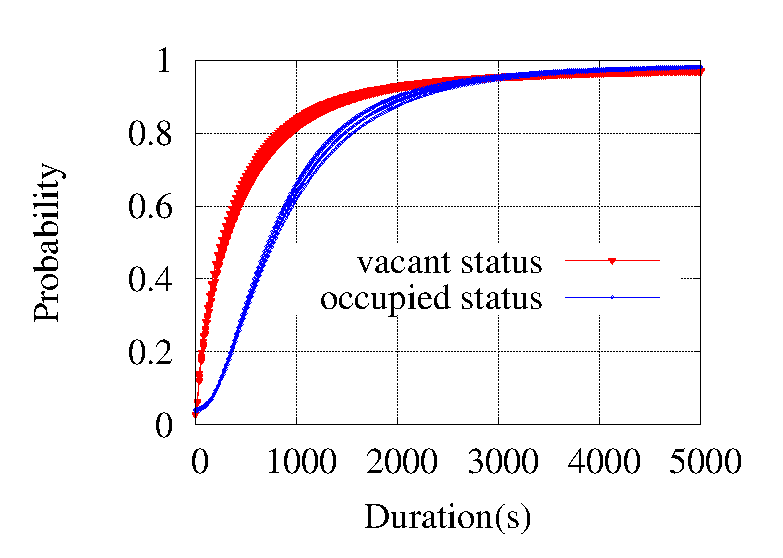
\includegraphics[width=0.5\textwidth]{figures/assumption/durationdis.eps}\\
\caption{状态持续时长分布}\label{figure_duration_for_each_status}
\end{figure}


\subsection{随时间变化的事件分布}


\begin{figure}[ht]
\centering
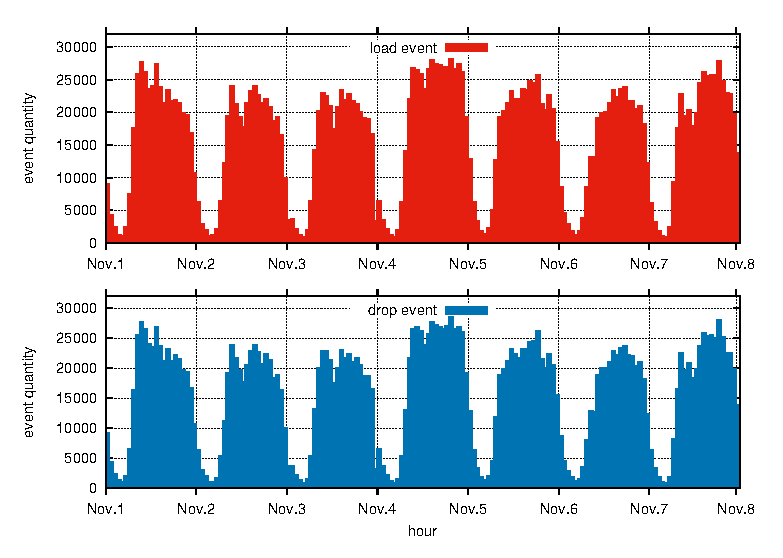
\includegraphics[width=0.65\textwidth]{figures/analysis/event_w_time.eps}\\
\caption{Taxi event varied with time.}\label{figure_event_varied_w_t}
\end{figure}



\begin{table}[ht]
\caption{随时间变化的事件数}\label{table_event_distribution_with_time}
\centering
\begin{tabular}{l|c|c}
 \hline
 名称 & 下客事件数 & 上客事件数 \\
  \hline
  一周总数& 2,679,385&2,707,290\\
  一小时内最大值&28,583 &28,130\\
  一小时内最小值&861&918\\
  波峰时段&11月4日, 19:00-20:00&11月4日, 19:00-20:00\\
  波谷时段&11月3日, 4:00-5:00&11月3日, 4:00-5:00\\
  \hline
  \end{tabular}
\end{table}




\begin{figure}[ht]
\centering
\fbox{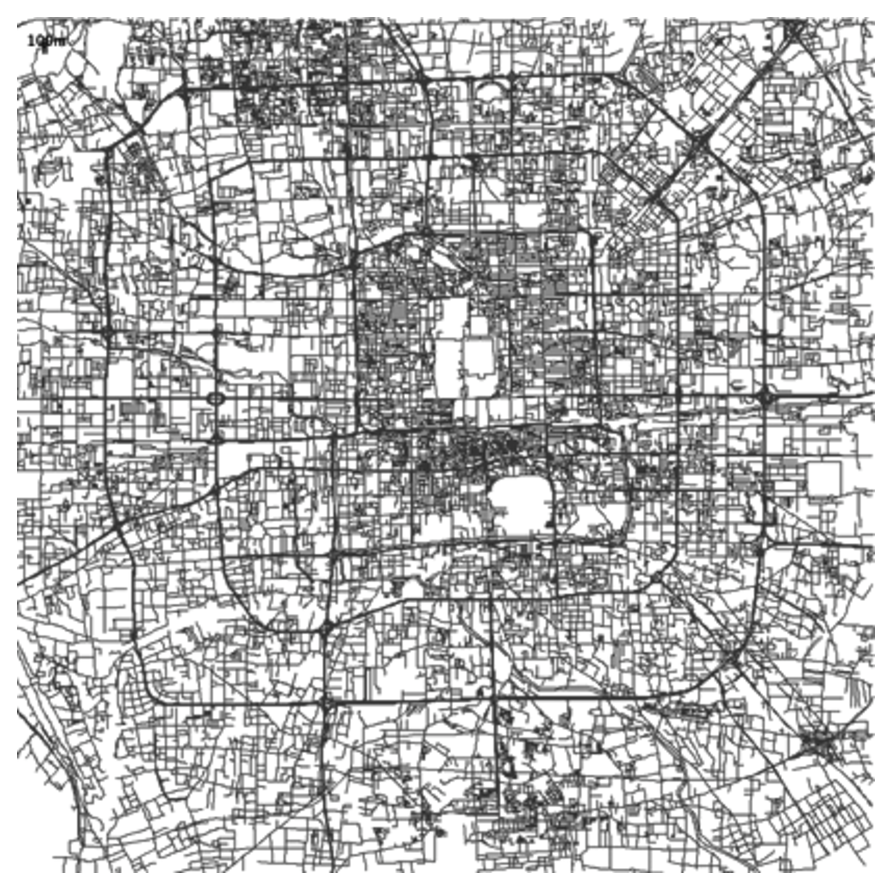
\includegraphics[width=0.4\textwidth]{figures/map.eps}}\\
\caption{抽取地图}\label{figure_map}
\end{figure}


\begin{figure}[ht]
\centering
\begin{tabular}
[c]{cc}
\epsfysize=2in\epsfbox{figures/analysis/hotspots/hotspot_drop_04.eps} &
\epsfysize=2in\epsfbox{figures/analysis/hotspots/hotspot_drop_19.eps} \\
(a) drop events at 4:00-5:00 & (b) drop events at 19:00-20:00\\
\epsfysize=2in\epsfbox{figures/analysis/hotspots/hotspot_load_04.eps} &
\epsfysize=2in\epsfbox{figures/analysis/hotspots/hotspot_load_19.eps} \\
(c) load events at 4:00-5:00 & (d) load events at 19:00-20:00\\
\end{tabular}
\caption{Taxi density for load/drop events in one hour.}\label{figure_taxi_density_for_one_hour}
\end{figure}


\begin{figure}[ht]
\centering
\begin{tabular}
[c]{cccc}
\epsfysize=1in\epsfbox{figures/analysis/hotspots/1hotspot_20_drop_19.eps} &
\epsfysize=1in\epsfbox{figures/analysis/hotspots/3hotspot_20_drop_19.eps} &
\epsfysize=1in\epsfbox{figures/analysis/hotspots/5hotspot_20_drop_19.eps} &
\epsfysize=1in\epsfbox{figures/analysis/hotspots/6hotspot_20_drop_19.eps} \\
(a) 11月1日,周二 &(b) 11月3日, 周四 &(c) 11月5日, 周六 &(d) 11月6日,周日 \\
\multicolumn{4}{c}{下客事件热点区域}\\
\epsfysize=1in\epsfbox{figures/analysis/hotspots/1hotspot_20_load_19.eps} & 
\epsfysize=1in\epsfbox{figures/analysis/hotspots/3hotspot_20_load_19.eps} &
\epsfysize=1in\epsfbox{figures/analysis/hotspots/5hotspot_20_load_19.eps} &
\epsfysize=1in\epsfbox{figures/analysis/hotspots/6hotspot_20_load_19.eps} \\
(e) 11月1日,周二 &(f) 11月3日, 周四 &(g) 11月5日, 周六 &(h) 11月6日,周日 \\
\multicolumn{4}{c}{载客事件热点区域}\\
\end{tabular}
\caption{出租车一小时内载客和下客事件的数量的区域分布}\label{figure_taxi_density_for_one_hour}
\end{figure}


\section{建立模型}

移动模型定义了节点的运动模式$Paths:<p_1,p_2…,p_n>$,$p_i$的确定可以简化为两步,即,目的地点选择和从源地点到目的地点的移动模式。
目的地点选择:节点的目的选择也与节点的当前状态有关。若节点处于载客状态。若当前状态为载客状态:针对载客事件将区域划分为不同的子区域,同理由下客事件分布将区域划分为不同的子区域。计算由载客子区域到下客子区域的转移概率矩阵和距离范围。然后由节点当前位置,决定下客位置。同理,节点处于下客状态时,由当前位置,和区域转移矩阵也可以计算得到载客的目的节点。


\subsection{区域定义与识别}
lalal


\subsection{区域转移概率}
区域转移概率


\subsection{时间建模}
time~


\subsection{速度建模}
\begin{figure}[!h]
\centering
\begin{tabular}
[c]{cc}
\multicolumn{2}{c}{6:00-8:00}\\
\epsfysize=1.5in\epsfbox{figures/evalue/fitspeed6_0.eps} &
\epsfysize=1.5in\epsfbox{figures/evalue/fitspeed6_1.eps} \\
\multicolumn{2}{c}{11:00-13:00}\\
\epsfysize=1.5in\epsfbox{figures/evalue/fitspeed11_0.eps} &
\epsfysize=1.5in\epsfbox{figures/evalue/fitspeed11_1.eps} \\
\multicolumn{2}{c}{17:00-19:00}\\
\epsfysize=1.5in\epsfbox{figures/evalue/fitspeed17_0.eps} &
\epsfysize=1.5in\epsfbox{figures/evalue/fitspeed17_1.eps} \\
\multicolumn{2}{c}{22:00-24:00}\\
\epsfysize=1.5in\epsfbox{figures/evalue/fitspeed22_0.eps} &
\epsfysize=1.5in\epsfbox{figures/evalue/fitspeed22_1.eps} \\
(a) vacant status & (b) occupied status \\
\end{tabular}
\caption{速度分布的拟合结果}\label{figure_fitspeed_varied_with_time}
\end{figure}



为了获取各个状态的速度分布,我们对瞬时速度的累积分布进行拟合,以获取瞬时速度的累积分布函数,然后衍生出其速度分布函数。
由图\ref{figure_fitspeed_varied_with_time}可知,除了载客状态时从22:00-24:00的累积瞬时速度分布外,瞬时速度的累积分布表现出指数分布的规律,拟合函数记为$f_1(x)$。载客状态时从22:00-24:00的累积瞬时速度分布表现出线性分布的特性,其拟合函数记为$f_2(x)$, 如公式\ref{formular_ccdf_speed}。由分析过程可知,某些天,例如周末的某些时段会影响车辆的行为,我们仅分析最常见的情况,因此去掉了明显不一样的情况,例如周六和周天早上6点到8点时的载客状态的累积速度分布。

\begin{equation}\label{formular_ccdf_speed}
\left\{
\begin{array}{ll}
f_1(x) = 1-1/exp(-ax^b-c)\\
f_2(x) = ax+b
\end{array}
\right.
\end{equation}

\begin{table}[ht]
\caption{拟合参数以及拟合曲线的残差平方和}\label{table_rms}
\centering
\begin{tabular}{c|c|c}
  \hline
  时间段 & 空车状态 & 载客状态 \\
  \hline
6:00-8:00   &0.0129207 & 0.019818 \\
11:00-13:00 &0.00866176 & 0.0204889 \\
17:00-19:00 &0.0176578 & 0.0105868 \\
22:00-24:00 &0.0154822 & 0.0240426 \\
  \hline
\end{tabular}
\end{table}

拟合结果以及相关的残差平方和(root mean square, rms)如表\ref{table_rms}所示,越小的残差平方和代表越小的误差。由表\ref{table_rms}可知,所有的残差平方和均小于$0.025$,表现出较好的拟合相似性。


\section{本章小结}
tete


\chapter{实验验证与结果分析}

本章根据之前的模型设计,结合仿真平台对所提出的基于海量交通数据的出租车移动模型进行了编码实现,并利用仿真平台对协议的性能进行了模拟验证,对比其与实际轨迹在接触和节点分布上的相似性,并与其他传统移动模型相比较。

\section{出租车移动模型的仿真实现}
\section{验证指标}
\section{接触验证}
\section{节点分布验证}
\section{本章小结}


In this section, T-START mobility model is validated on the aspects of node distribution compared with existing mobility models and the real traces. We pick two simple mobility models for comparison: one free space - Random Way Point (RWP) model, the other is constrained model, Shortest Path (SP).  SP mobility model is based on the underlying map of Beijing where vehicles move along the map roads by Dijkstra algorithm to random destinations. Both models take no consideration of the node statuses. All mobility models are implemented on Opportunistic Networking Environment (ONE)\cite{KeranenOtt-155}.

In our simulations, vehicles are deployed in an area of $24,000\times 24,000 m^2$, including fourth ring roads in Beijing.
To evaluate the time feature of T-START, 4 time periods are chosen: in the morning from 6:00:00 to 7:59:59, at noon from 11:00 to 13:00, at afternoon from 17:00 to 19:00 and lat in the evening from 22:00 to 24:00. Accordingly, we extract the real traces at corresponding time period of 21st November 2011.
3000 taxies are randomly selected. 
We need to configure the speed range for RWP and SP mobility model. Those two models will generate a new speed randomly in the speed range. We set the speed range from 0 to twice the average speed for certain time period.
The average speed for RWP and SP are set as $15.83km/h$ for 6:00 to 8:00, $18.43km/h$ for 11:00 to 13:00, $15.25km/h$ for 17:00 to 19:00 and $20.46km/h$ for 22:00 and 24:00. 
Thus, the speed ranges for the four time periods are $[0, 36.86]km/h$, $[0, 36.86]km/h$, $[0, 30.50]km/h$ and $[0, 40.802]km/h$.

\begin{figure}[h]
\centering
\subfigure[Real Trace]{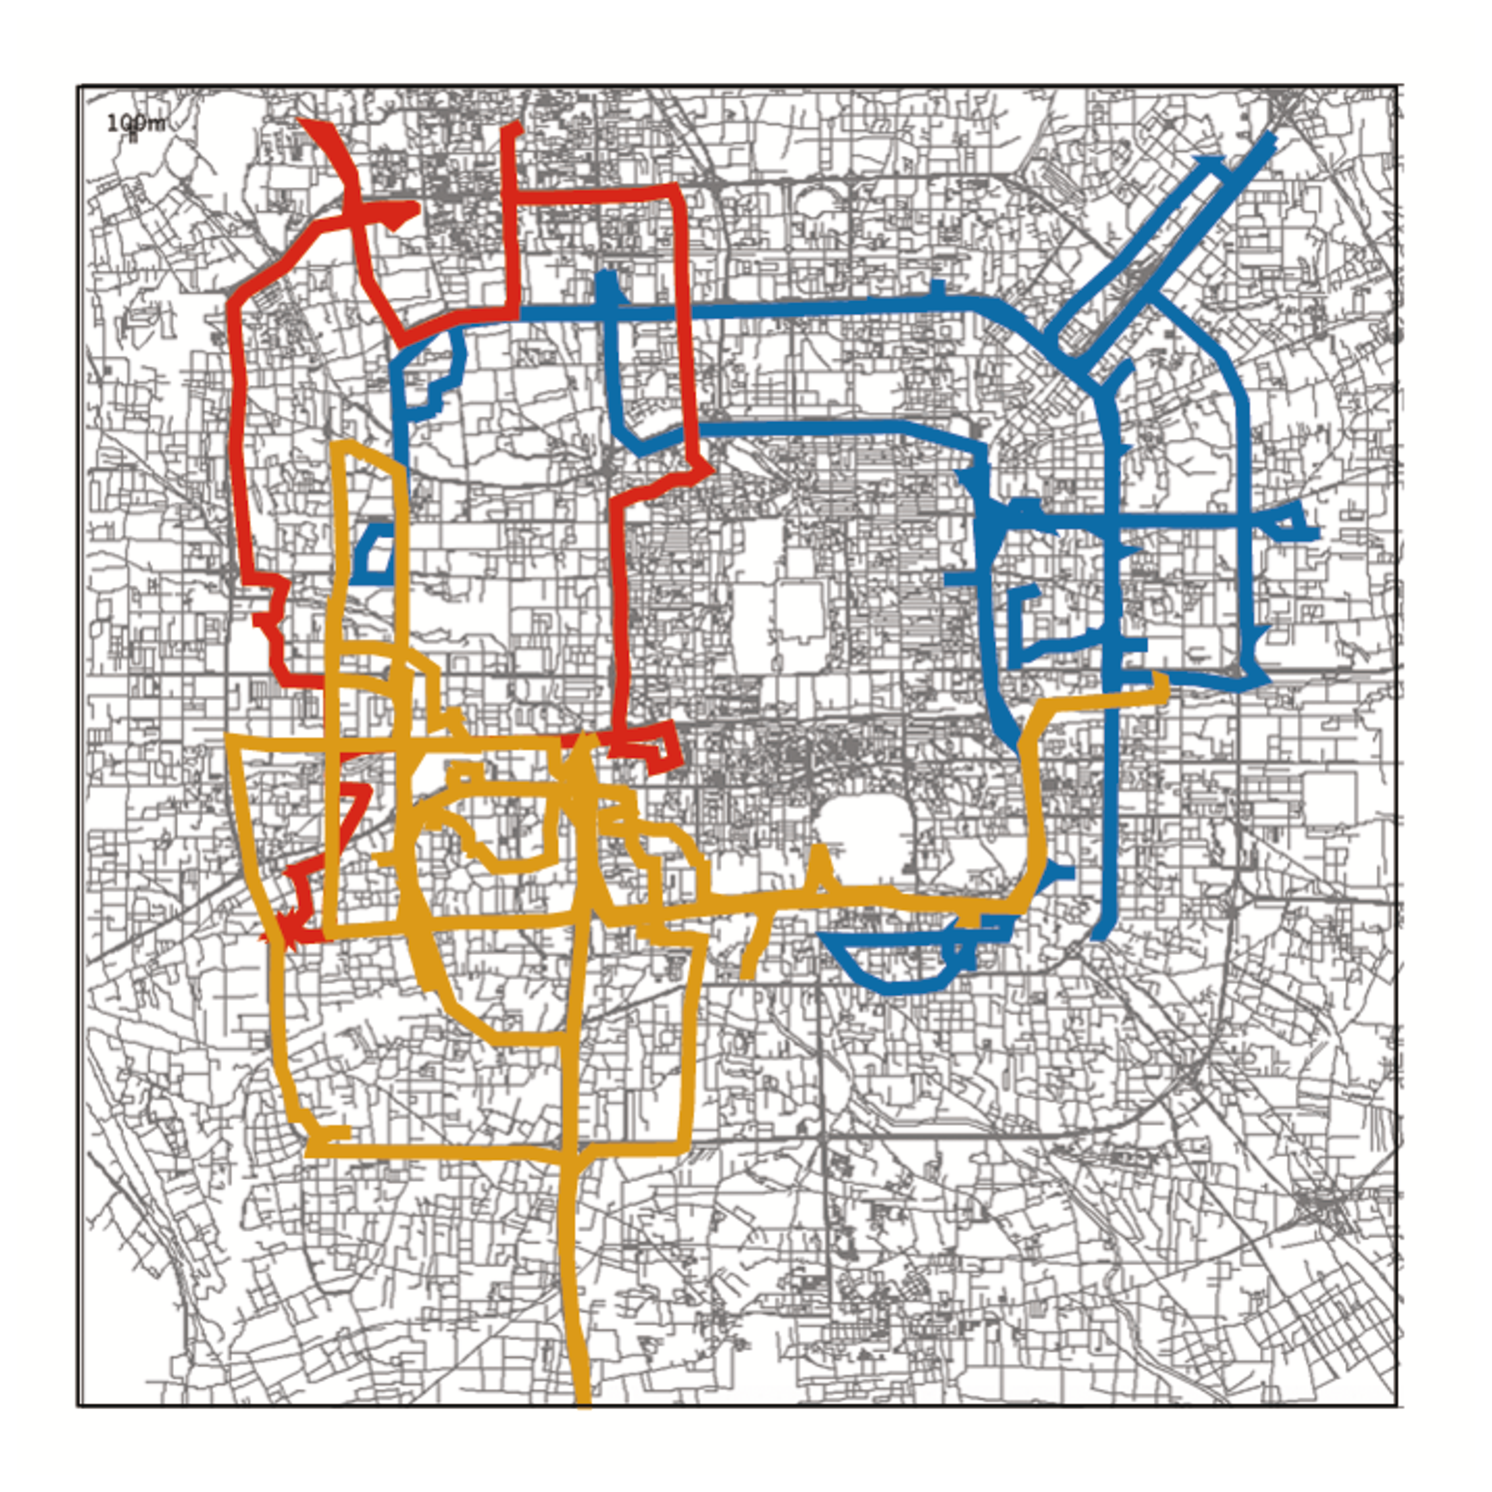
\includegraphics[width=0.24\textwidth]{figures/evalue/sample/real_traces.eps}}
\subfigure[T-START]{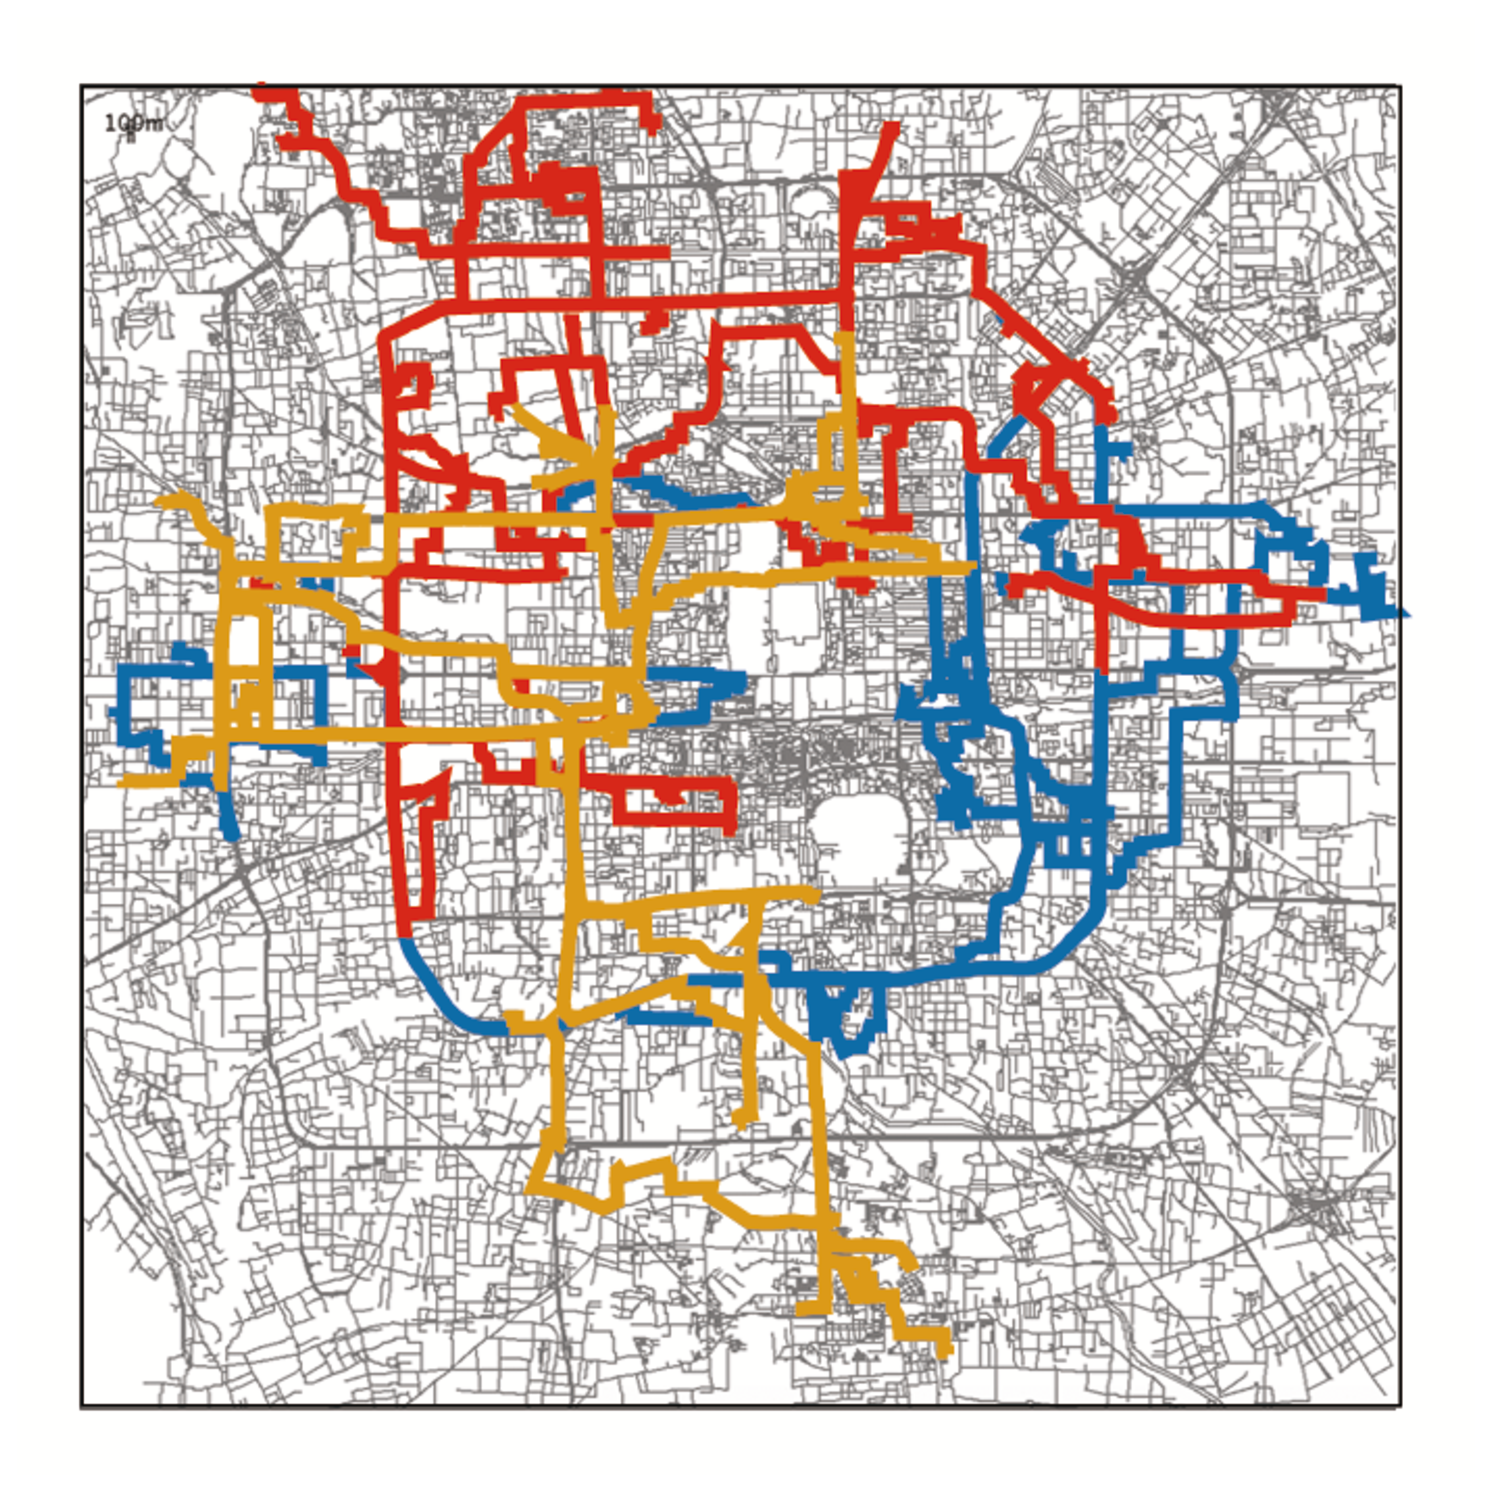
\includegraphics[width=0.24\textwidth]{figures/evalue/sample/start_traces.eps}}
\subfigure[SP]{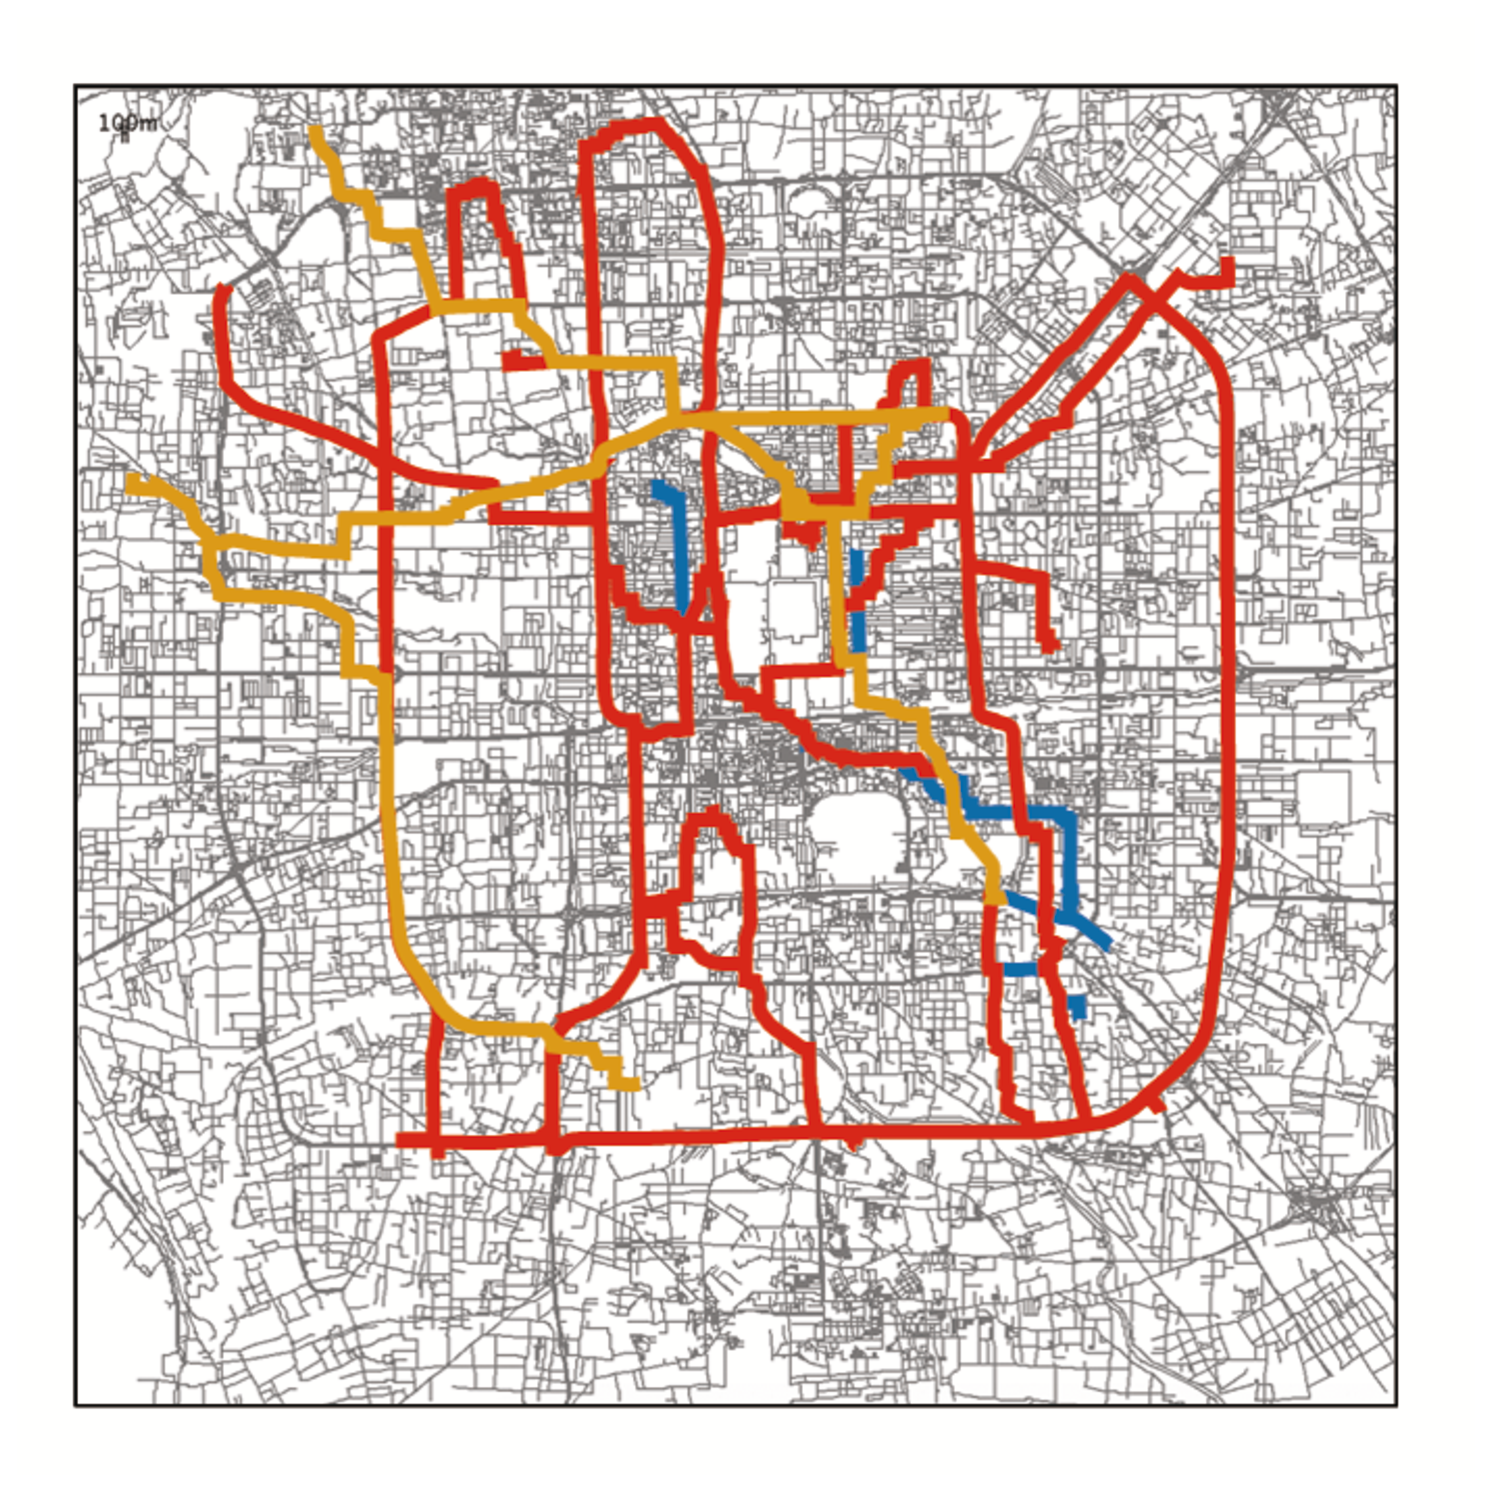
\includegraphics[width=0.24\textwidth]{figures/evalue/sample/sp_traces.eps}}
\subfigure[RWP]{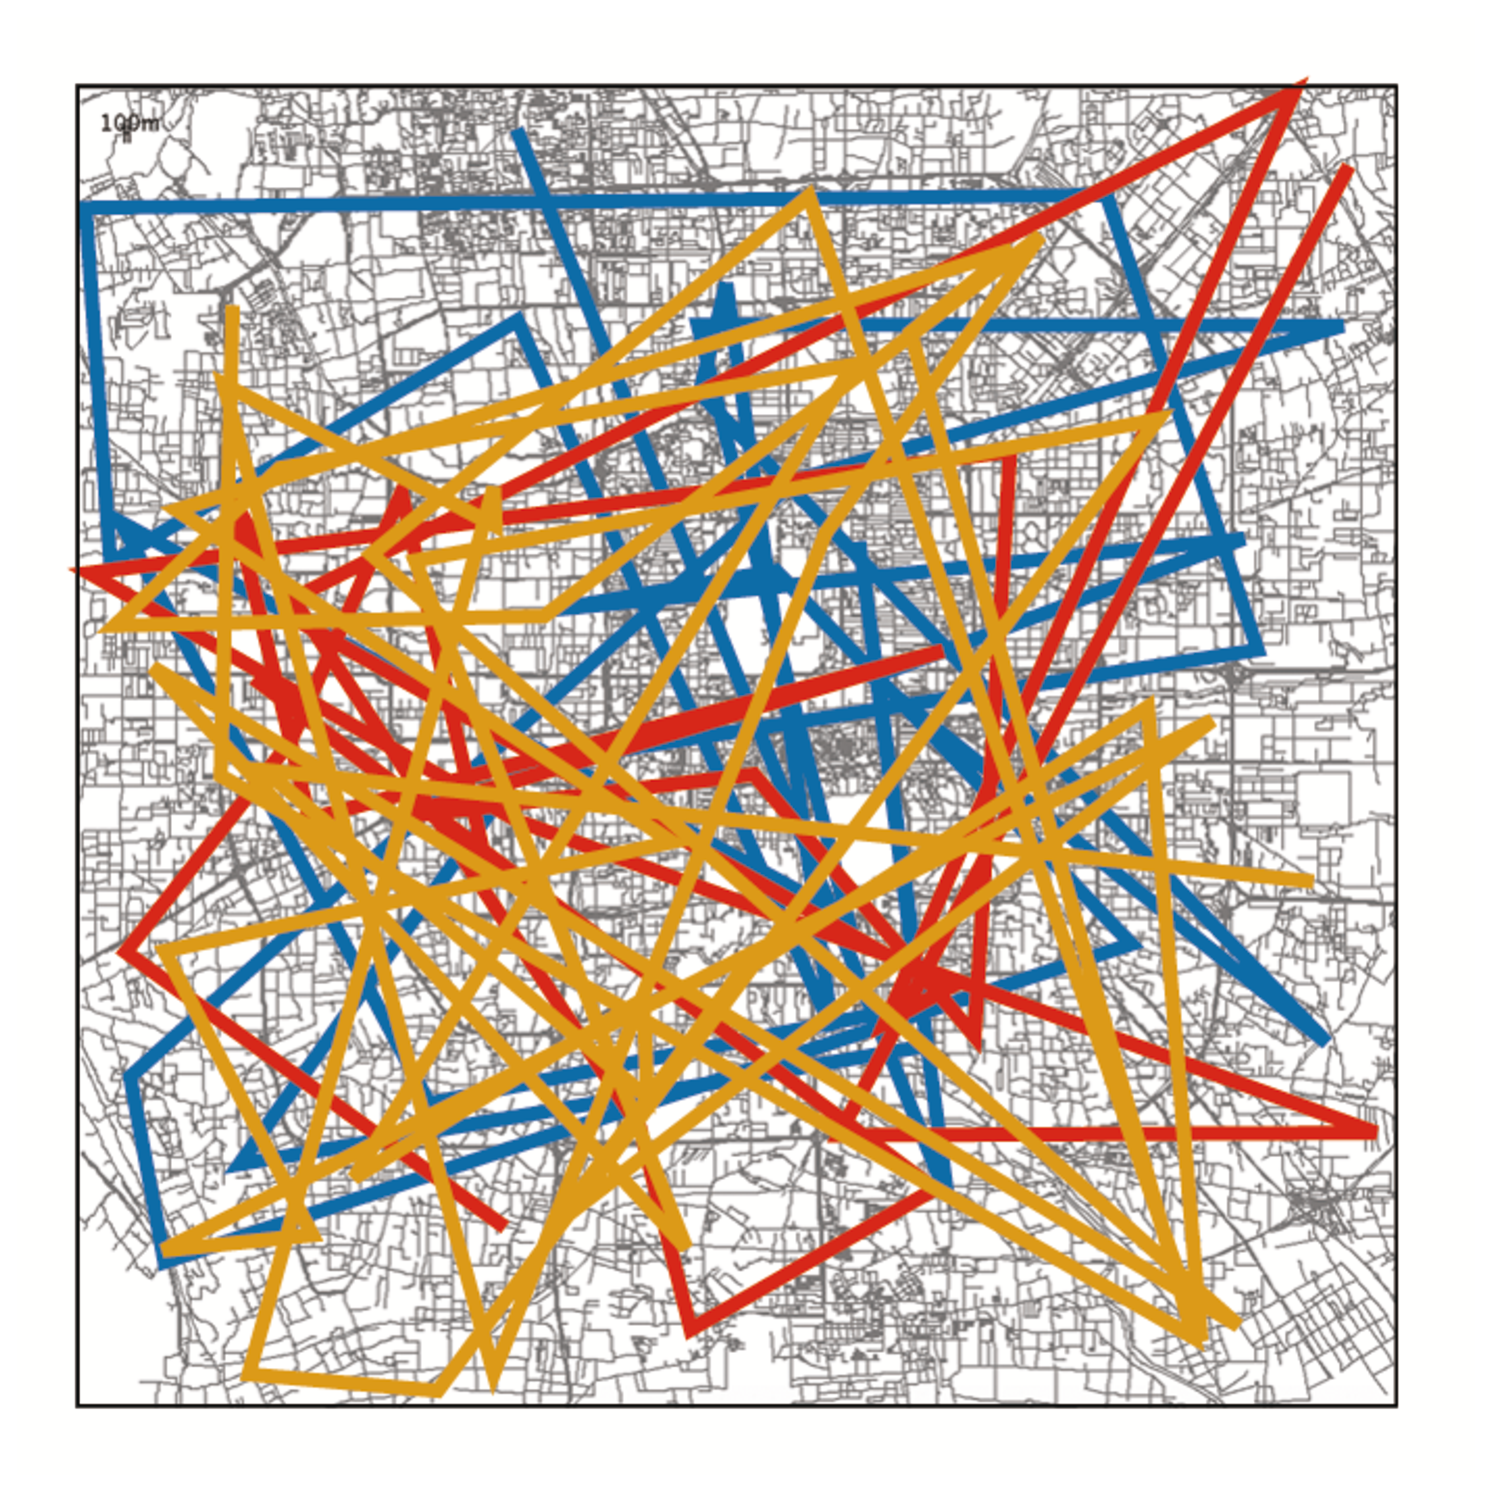
\includegraphics[width=0.24\textwidth]{figures/evalue/sample/rwp_traces.eps}}
\caption{模型生成的轨迹样例}\label{figure_tracesample}
\end{figure}

\begin{figure}[h]
\centering
\subfigure[Real Trace]{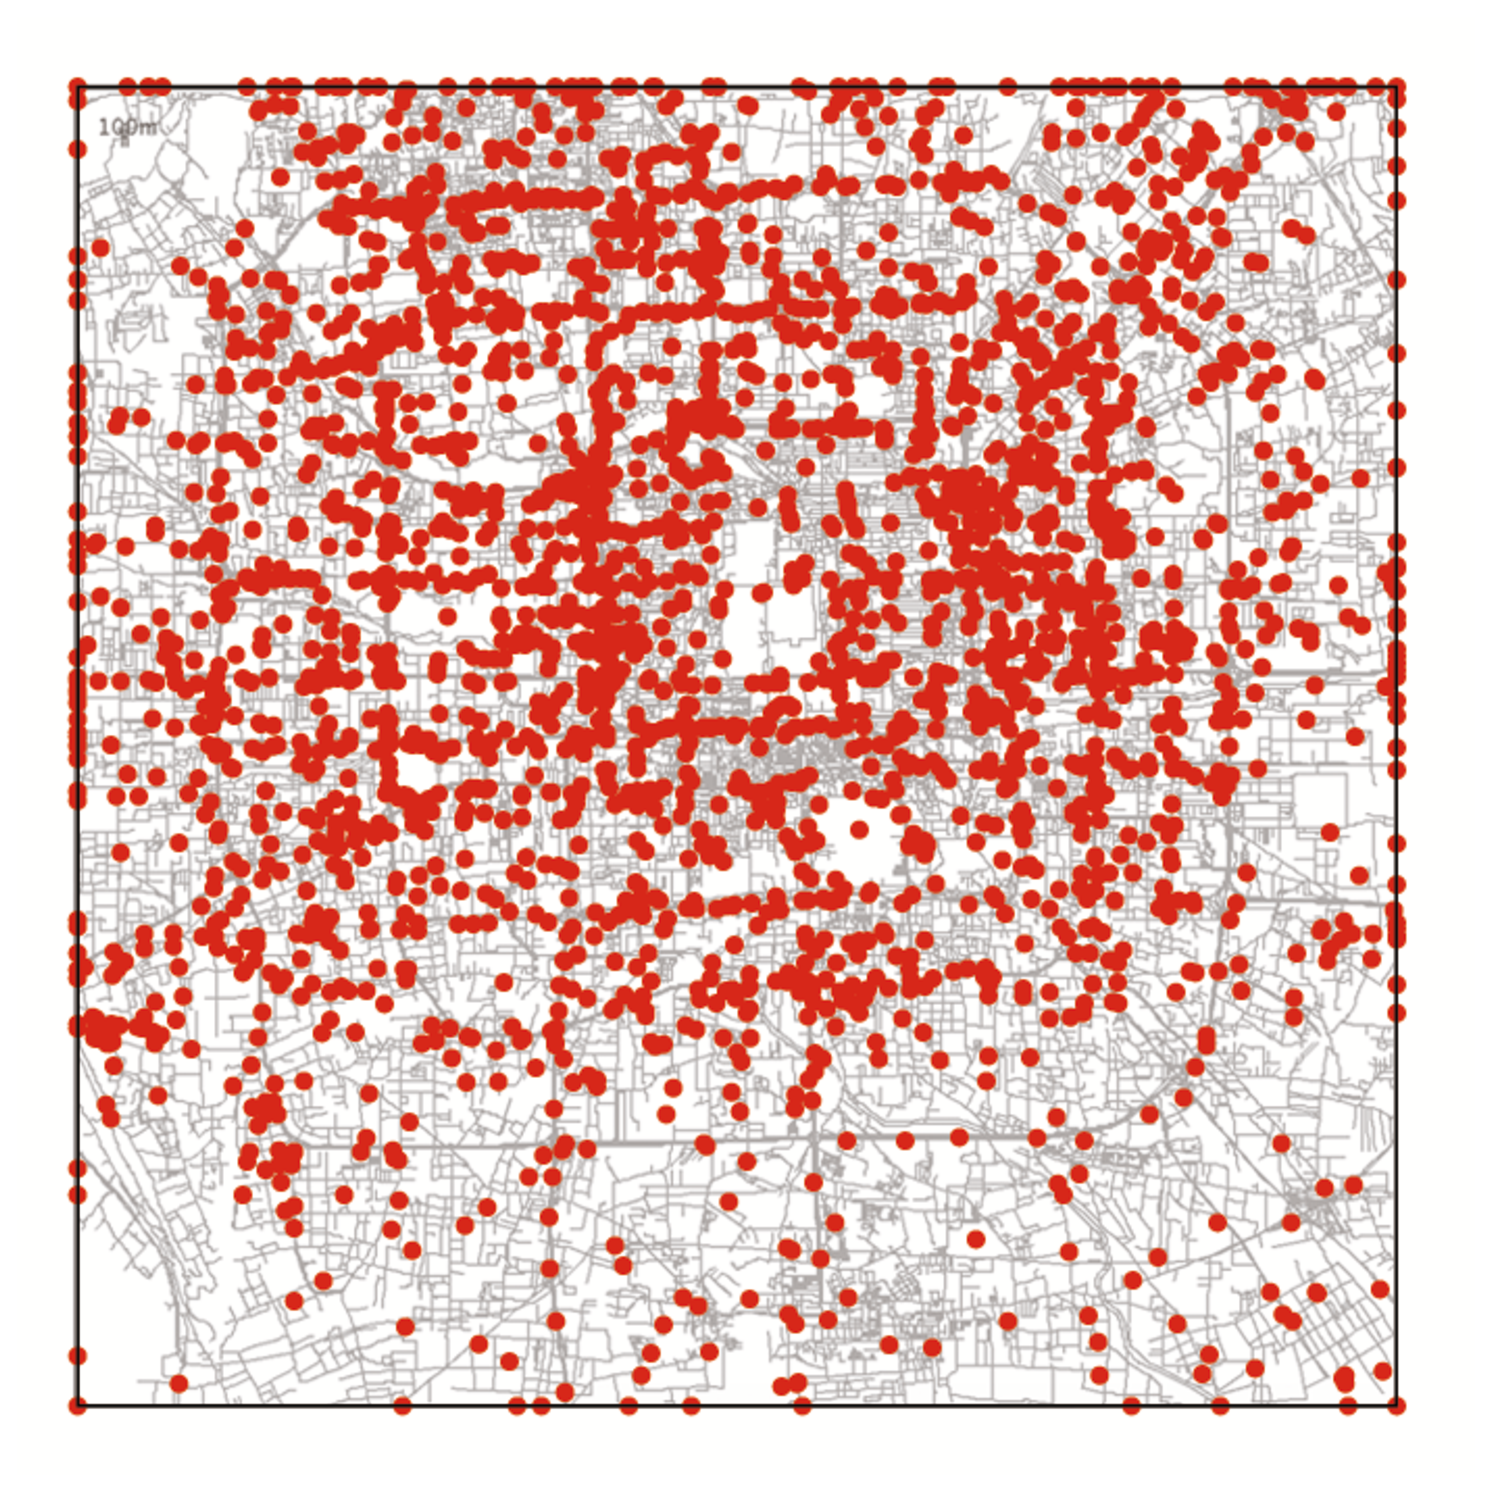
\includegraphics[width=0.24\textwidth]{figures/evalue/trace_nodedis.eps}}
\subfigure[T-START]{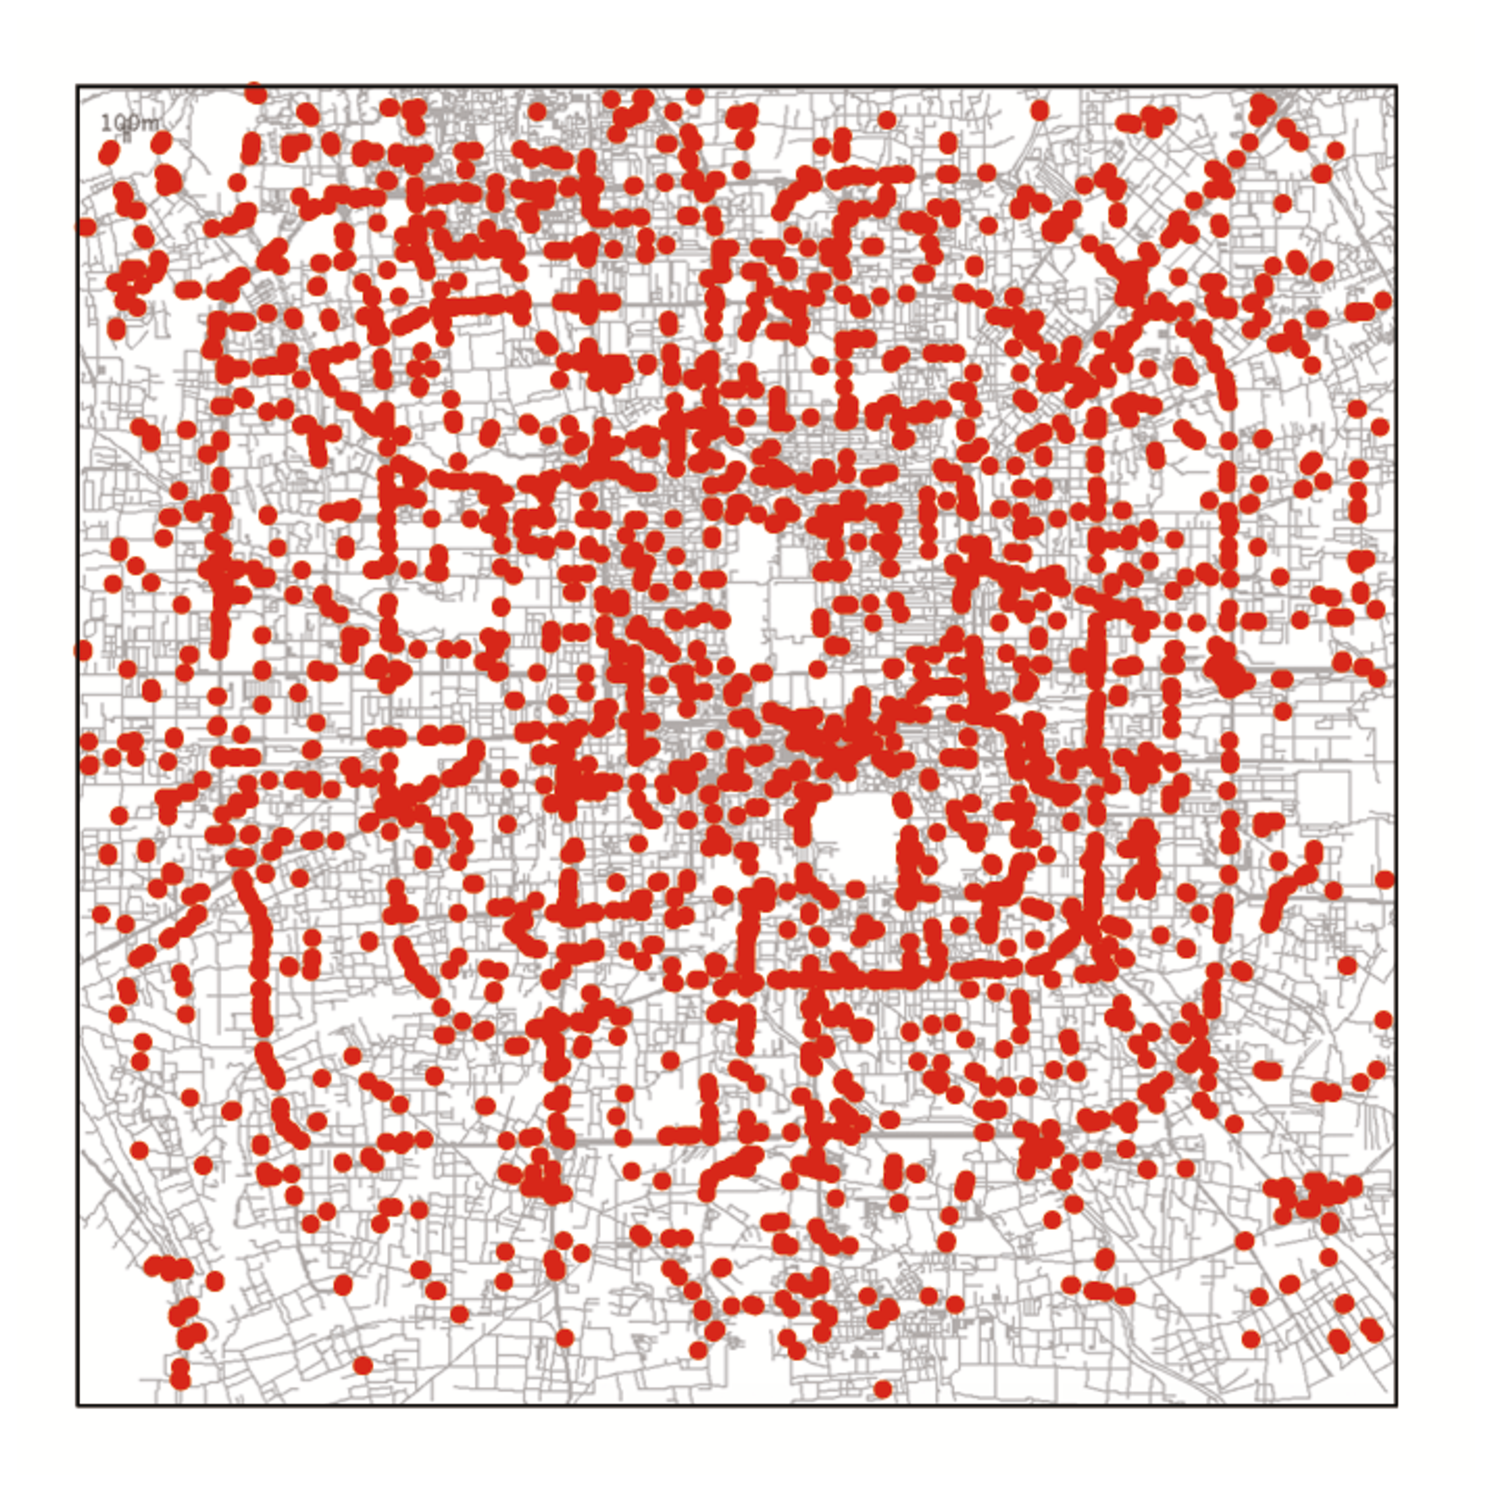
\includegraphics[width=0.24\textwidth]{figures/evalue/start_nodedis.eps}}
\subfigure[SP]{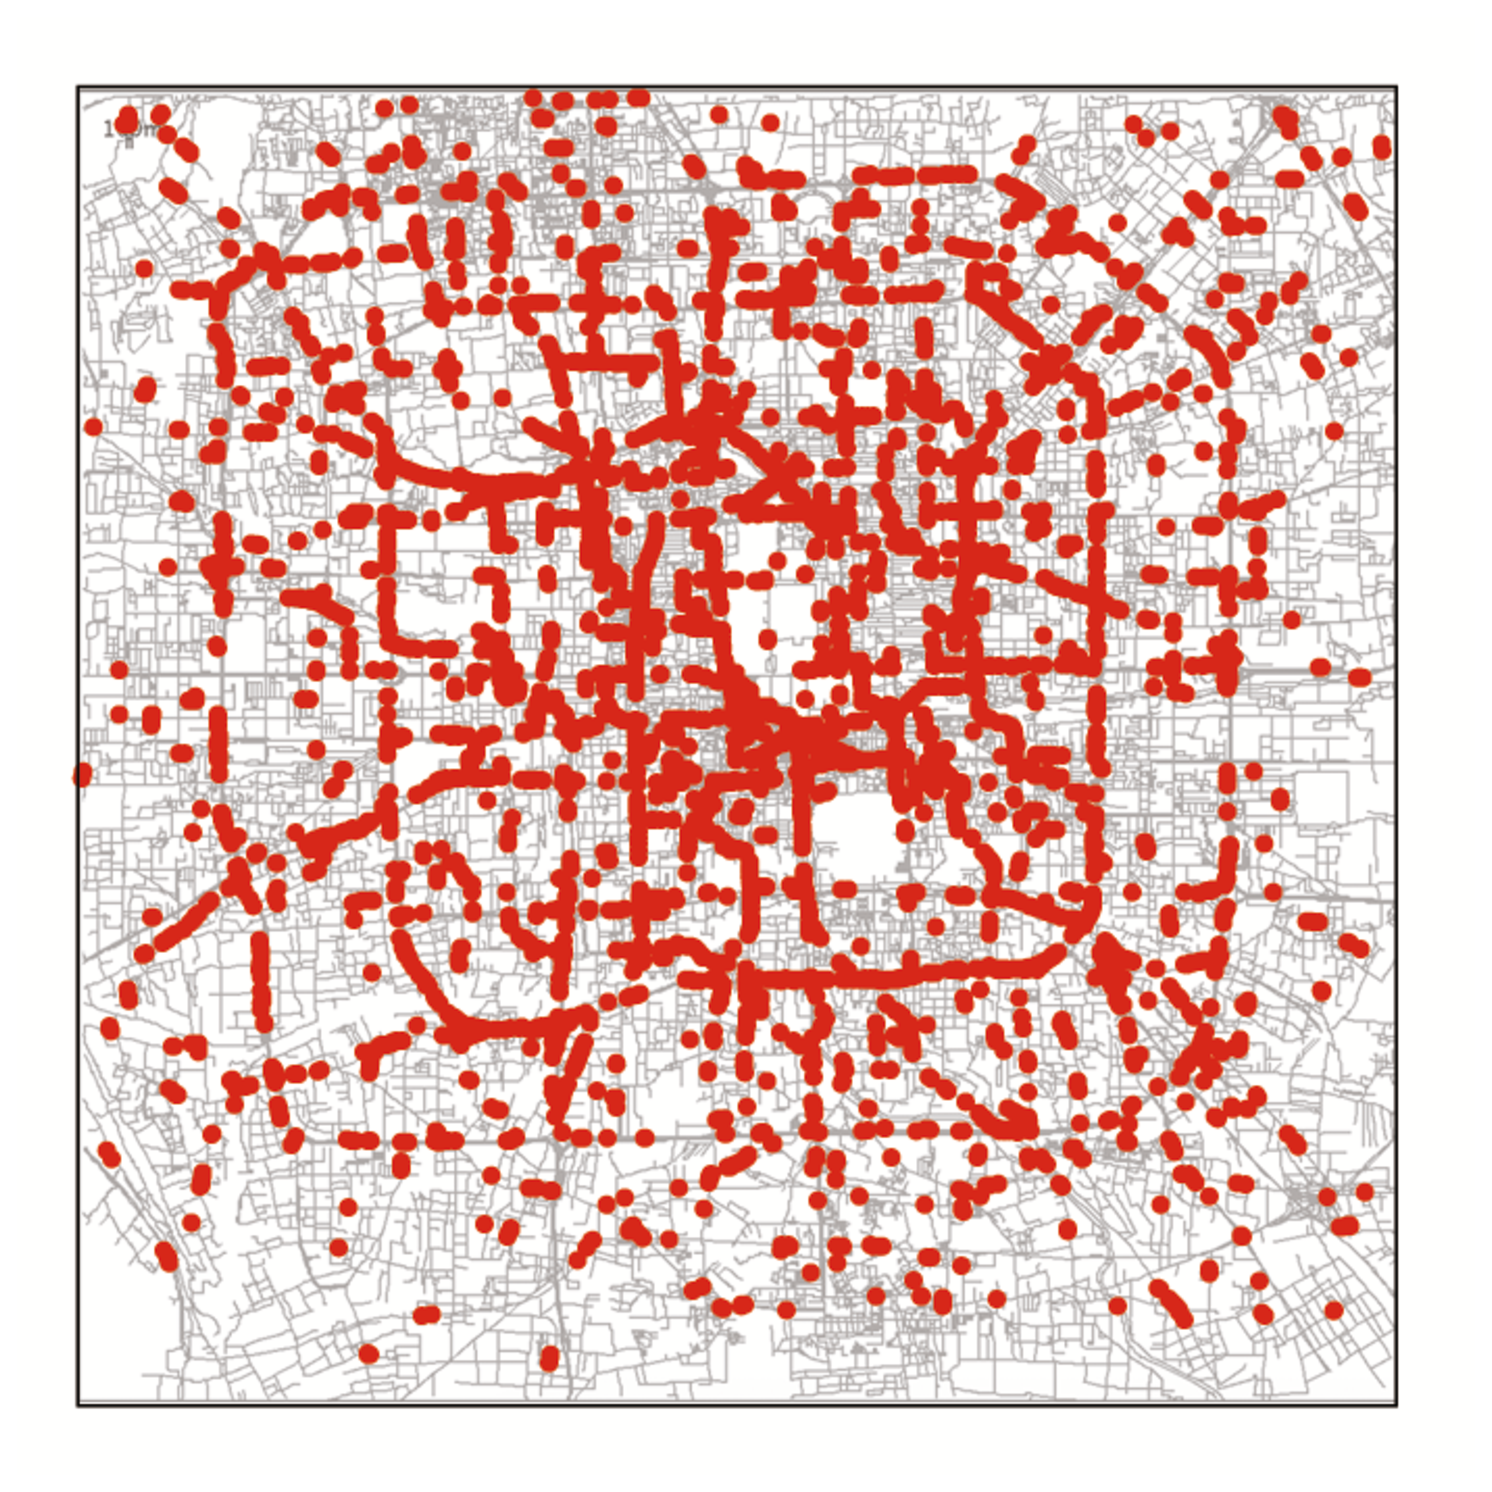
\includegraphics[width=0.24\textwidth]{figures/evalue/sp_nodedis.eps}}
\subfigure[RWP]{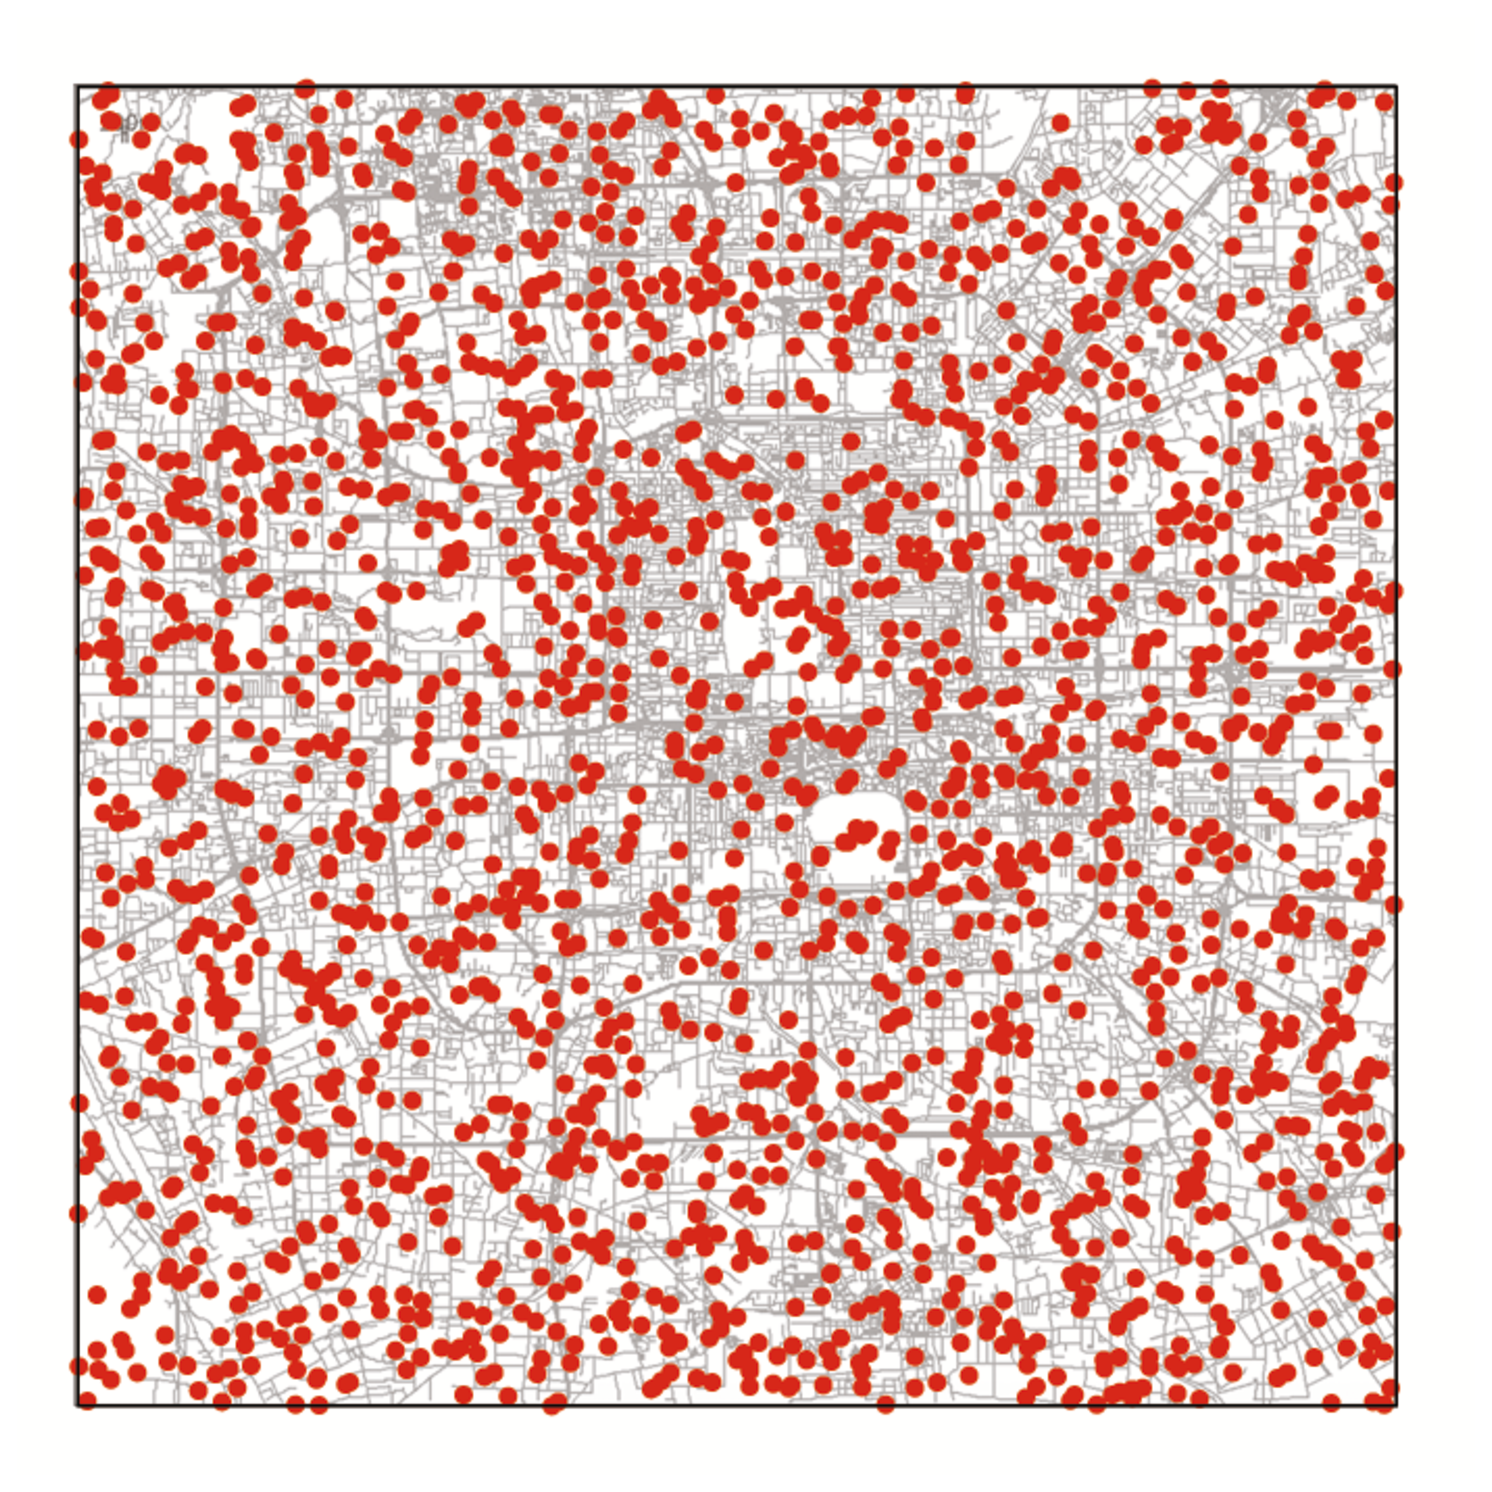
\includegraphics[width=0.24\textwidth]{figures/evalue/rwp_nodedis.eps}}
\caption{模型节点分布快照}\label{figure_trace_snapshots}
\end{figure}

Trace samples and their node distribution snapshots from different mobility models are reported in Fig.~\ref{figure_tracesample} and Fig~\ref{figure_trace_snapshots}. Fig.~\ref{figure_tracesample} shows the trace in one day. The traces of the real data and T-START only cover some parts of the area, while the traces of SP and RWP almost go through the whole area. Recall that SP and RWP select a destination randomly in the area, while T-START takes the associations between current region and destinations into consideration (which satisfies the movement rules of taxis). In Fig.~\ref{figure_trace_snapshots}, real trace, T-START and SP exhibit the road structures, while the node distribution of RWP is much uniform. As to T-START, the destination section process decides that it tends to select a destination in the regions with higher load/drop event probability. Therefore, with the decline of the randomness, the snapshot of T-START becomes much clear and centralized on the main roads, which matches real traces very well.
Since the node distribution has a great impact on the transport and network performance, a good understanding of it can help to route and control.  However, nodes are dynamic leading to a dynamic node distribution. In order to quantify the changing node distribution,  we introduce the in/out degree. The in/out degree figures out how many taxies moving in or out from a region in a time period. In/out degree defines how many nodes moveing in or out a area during a period of time. 
We divide the simulation scenario into grids of $ 400m \times 400 m$ to investigate the in/out degree, and the time period to measure the in/out degree is as two hours according to the simulation time. 
The average in-degree is equal to the average of out-degree. Because if a node moves out from area A to area B, the in-degree of B adds on one, meanwhile, the out-degree of area A adds on one. The average in/out degree are shown as table \ref{table_avg_inoutdegree}, and the variance of in-degree and out-degree are shown as table \ref{table_variance}.
We can figure out that the average in/out-degree for T-START and SP are similar with the Trace but that of RWP is relatively small. As to the variance of in/out-degree, from 6:00 to 8:00, the variance of T-START and SP are similar, however, the variance of T-START is larger than that of SP and more close to that of the real trace.  
\begin{figure}[!h]
\centering
\subfigure[average]{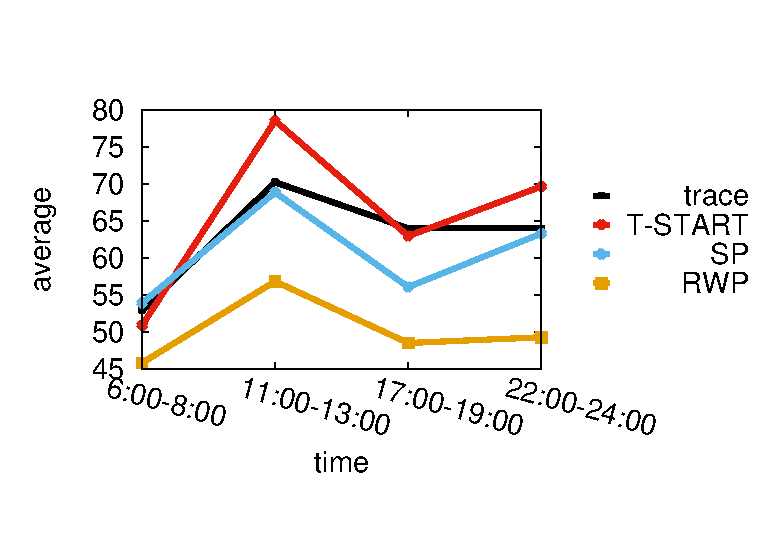
\includegraphics[width=0.5\textwidth]{figures/evalue/indegree/avg.eps}}
\subfigure[variance of in-degree]{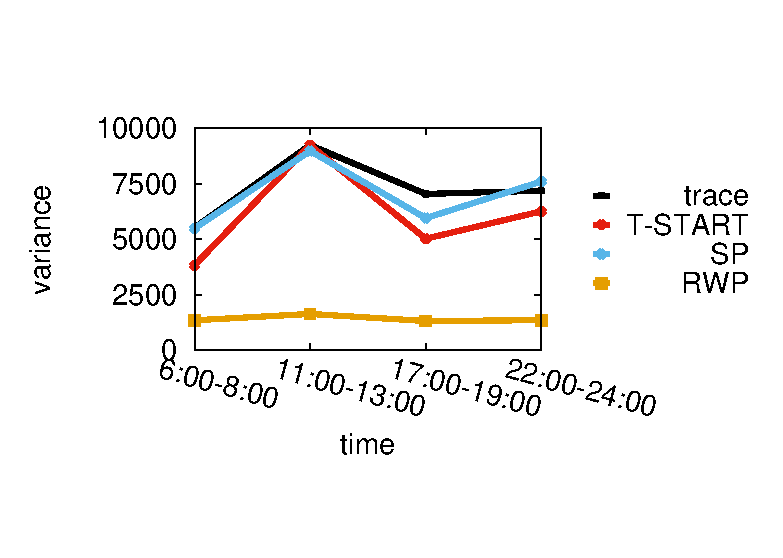
\includegraphics[width=0.5\textwidth]{figures/evalue/indegree/var_in.eps}}
\subfigure[variance of out-degree]{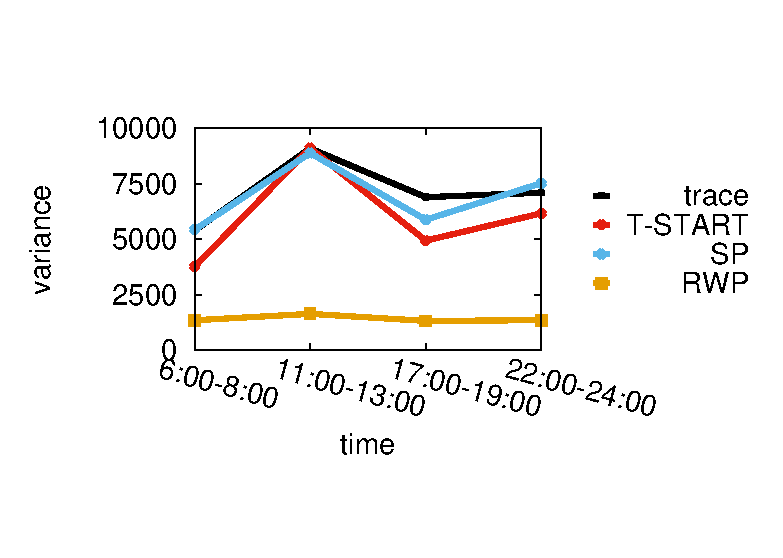
\includegraphics[width=0.5\textwidth]{figures/evalue/indegree/var_out.eps}}
\caption{出入度的均值和方差}\label{figure_avg}
\end{figure}


The in/out-degree distribution for the four time periods are ploted as figure \ref{figure_indegree_dis}.
For the RWP is similar, as figure \ref{figure_indegree_rwp}. We focus on the real trace, T-START and SP.  
From figure \ref{figure_indegree_dis}, the peaks of the real traces are contentrated on the main roads. For the T-START and SP use the Dijkstra algrothrithm, they will choose the shortest way to a destination, ignoring the factors of road condition. Nevertheless, we can find out some differences between T-START and SP. The peaks of indegree gather in the middle, because it chose the destination in a random way, while those of T-START distributes more to the ring roads.
\begin{figure}[h]
\centering
\epsfysize=2in\epsfbox{figures/evalue/indegree/17indegree_rwp.eps} 
\caption{从17:00 到 19:00 RWP的入度分布图}\label{figure_indegree_rwp}
\end{figure}
\begin{figure}[h]
\centering
\begin{tabular}
[c]{ccc}
\epsfysize=1.2in\epsfbox{figures/evalue/indegree/6indegree_trace.eps} &
\epsfysize=1.2in\epsfbox{figures/evalue/indegree/6indegree_start.eps} &
\epsfysize=1.2in\epsfbox{figures/evalue/indegree/6indegree_sp.eps} \\
\epsfysize=1.2in\epsfbox{figures/evalue/indegree/11indegree_trace.eps} &
\epsfysize=1.2in\epsfbox{figures/evalue/indegree/11indegree_start.eps} &
\epsfysize=1.2in\epsfbox{figures/evalue/indegree/11indegree_sp.eps} \\
\epsfysize=1.2in\epsfbox{figures/evalue/indegree/17indegree_trace.eps} &
\epsfysize=1.2in\epsfbox{figures/evalue/indegree/17indegree_start.eps} &
\epsfysize=1.2in\epsfbox{figures/evalue/indegree/17indegree_sp.eps} \\
\epsfysize=1.2in\epsfbox{figures/evalue/indegree/22indegree_trace.eps} &
\epsfysize=1.2in\epsfbox{figures/evalue/indegree/22indegree_start.eps} &
\epsfysize=1.2in\epsfbox{figures/evalue/indegree/22indegree_sp.eps} \\
(a) Traces of Nov.8th & (b) T-START & (c) SP \\
\end{tabular}
\caption{实际轨迹, T-START和SP的入度分布图}\label{figure_indegree_dis}
\end{figure}
In order to quantity the similarity between the mobility models and the real traces, we introduce the conception of the relative error. 
The relative error is calculated as:
\begin{equation}
    \delta = \frac{\sum \Delta x}{\sum x_{real}} 
\end{equation}
$\Delta x$ is the absolute value of the compare value minus the real one, and $x_{real}$ is the real value.

Firstly, in order to find out the relative error is valid, we extracted the in/out-degree matrixes from November 1 to November 7 for the four time periods, and then obtain a average matrix for every time period. Then, we compare the in/out-degree of every single day of the seven days with the average matrix, the results are shown as table \ref{table_relative_err_avg}. The relative error between every day with corresponding matrix are in a range from 0.1 to 0.25. It shows that the in/out-degree distributions for different time periods have certain regularity and we can utilize the average matrix for corresponding time as a comparition. 
\begin{table}[!t]
\centering
\caption{The relative error compared with the average for in-degree and out-degree}\label{table_relative_err_avg}
\begin{tabular}[c]{c|c|c|c|c|c|c|c}
\multicolumn{8}{c}{(a) in-degree}\\
\hline
item& 1th&2th&3th&4th&5th&6th&7th\\
\hline
6:00-8:00&
0.1139& 
0.1485&
0.1732&
0.1372&
0.1500&
0.2489&
0.1507\\
11:00-13:00&
0.1056&
0.0953&
0.1509&
0.0994&
0.1714&
0.1294&
0.1011\\
17:00-19:00&
0.1537&
0.1728&
0.1491&
0.1888&
0.1338&
0.1303&
0.1407\\
22:00-24:00&
0.1360&
0.1054&
0.1637&
0.1183&
0.1467&
0.1470&
0.1076\\
\hline
\end{tabular}
\begin{tabular}[c]{c|c|c|c|c|c|c|c}
\multicolumn{8}{c}{(b) out-degree}\\
\hline
item& 1th&2th&3th&4th&5th&6th&7th\\
\hline
6:00-8:00&
0.1132&
0.1481&
0.1726&
0.1374&
0.1499&
0.2478&
0.1507\\
11:00-13:00&
0.1057&
0.0953&
0.1509&
0.0998&
0.1719&
0.1296&
0.1012\\
17:00-19:00&
0.1534&
0.1725&
0.1488&
0.1890&
0.1336&
0.1298&
0.1412\\
22:00-24:00&
0.1358&
0.1057&
0.1636&
0.1184&
0.1468&
0.1469&
0.1075\\
\hline
\end{tabular}
\end{table}
Therefore, compare of the average in/out-degree matrix, the relative errors of the trace of Nov.8th, T-START, SP and RWP are shown as table \ref{table_relative_err}.
The relative error of the trace of Nov.8th remains in a low level about 0.1.
The relative error of T-START is about 0.48, while that of SP is about 0.65 and RWP is more than 0.8 for every time period.  

\begin{figure}[ht]
\centering
\subfigure[relative error of in-degree]{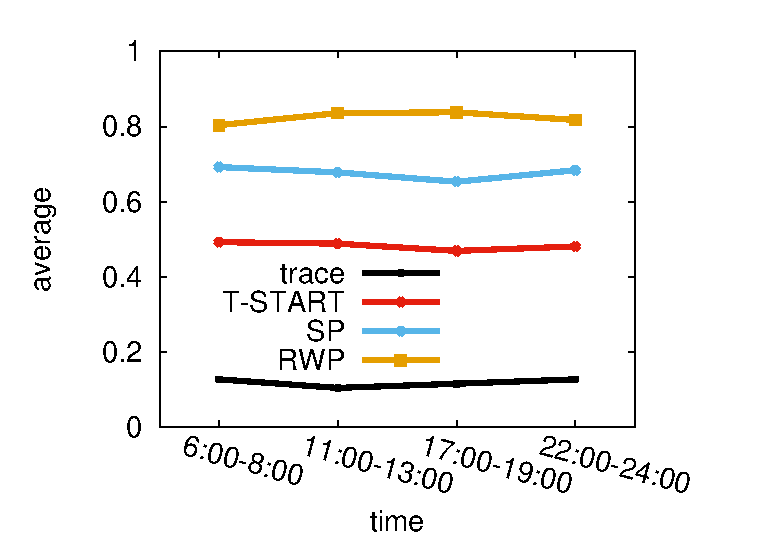
\includegraphics[width=0.45\textwidth]{figures/evalue/indegree/err_in.eps}}
\subfigure[relative error of out-degree]{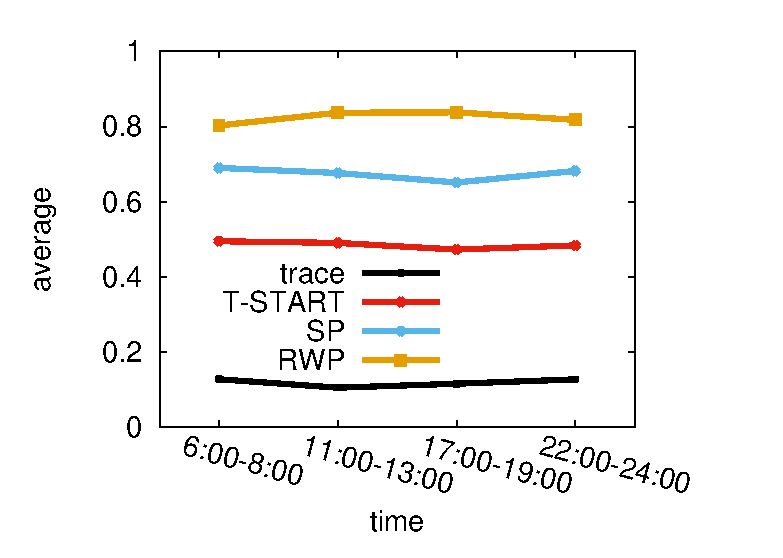
\includegraphics[width=0.45\textwidth]{figures/evalue/indegree/err_out.eps}}
\caption{average and variance of in/out-degree.}\label{figure_avg}
\end{figure}

\chapter{总结与展望}



%选题背景与意义
%文献以及相关综述
%建模过程i
%验证
%结论

%\include{data/chapter1-intro}
%\include{data/chapter2-config}
%\include{data/chapter3-download}
%\include{data/chapter4-basic}
%\include{data/chapter5-usage}
%\include{data/chapter6-implement}
%\include{data/chapter7-conclusion}

% 参考文献
\include{data/reference}

% 附录
\appendix
% !Mode:: "TeX:UTF-8"
\chapter{区域识别算法伪代码}
\begin{algorithm}\label{algorithm_connecting}
\caption{Clustering}
\begin{algorithmic}
\STATE \textbf{INPUTs:} $Cells=\{C_{x,y}\}$, the event threshold $\eta$, 
$CLUSTERSCALE$, and $REGIONSEED=200$.\\
\STATE $ClusterQueue=\varnothing$ \& $UsedCells=\varnothing$\\
\STATE Sort $Cells$ by events in descending order\\
\FOR{$CELL_{x,y}\in Cells$}
\IF{$CELL_{x,y}\notin UsedCells$}
\STATE¡¡$CELL_{x,y}.region=REGIONSEED$\\
\STATE  $size=1$\\
\STATE  $CLUSTERSEED=CLUSTERSEED-1$\\
\STATE $ClusterQueue.enqueue(CELL_{x,y})$
\STATE $UsedCells.add(CELL_{x,y})$
\WHILE{$ClusterQueue \neq \varnothing$}
\STATE $CELL_{x,y}=ClusterQueue.dequeue()$
\IF{$REGIONSEED\geq0$ \AND $CELL_{x,y}.events\geq\eta$}
\STATE $enqueueNeighbor(CELL_{x-1,y})$
\STATE $enqueueNeighbor(CELL_{x-1,y-1})$
\STATE $enqueueNeighbor(CELL_{x-1,y+1})$
\STATE $enqueueNeighbor(CELL_{x+1,y})$
\STATE $enqueueNeighbor(CELL_{x+1,y-1})$
\STATE $enqueueNeighbor(CELL_{x+1,y+1})$
\STATE $enqueueNeighbor(CELL_{x,y-1})$
\STATE $enqueueNeighbor(CELL_{x,y+1})$
\ELSE
\STATE $enqueueNeighborOthers(CELL_{x-1,y})$
\STATE $enqueueNeighborOthers(CELL_{x-1,y+1})$
\STATE $enqueueNeighborOthers(CELL_{x-1,y-1})$
\STATE $enqueueNeighborOthers(CELL_{x+1,y})$
\STATE $enqueueNeighborOthers(CELL_{x+1,y-1})$
\STATE $enqueueNeighborOthers(CELL_{x+1,y+1})$
\STATE $enqueueNeighborOthers(CELL_{x,y-1})$
\STATE $enqueueNeighborOthers(CELL_{x,y+1})$
\ENDIF
\ENDWHILE
\ENDIF
\ENDFOR
\end{algorithmic}
\end{algorithm}



\begin{algorithm}
\caption{$enqueueNeighbor(CELL_{x,y})$}
\begin{algorithmic}
\IF{$CELL_{x,y}.events\geq \eta$ \AND $size<CLUSTERSCALE$ \AND $CELL_{x,y}\notin UsedCells$}
\STATE $ClusterQueue.enqueue(CELL_{x,y})$
\STATE¡¡$CELL_{x,y}.region=REGIONSEED$
\STATE $UsedCells.add(CELL_{x,y})$
\STATE $size=size+1$
\ENDIF
\end{algorithmic}
\end{algorithm}

\begin{algorithm}
\caption{$enqueueNeighborOthers(CELL_{x,y})$}
\begin{algorithmic}
\IF{$size<CLUSTERSCALE$\AND $CELL_{x,y}\notin UsedCells$}
\STATE $ClusterQueue.enqueue(CELL_{x,y})$
\STATE¡¡$CELL_{x,y}.region=REGIONSEED$\\
\STATE $UsedCells.add(CELL_{x,y})$
\STATE $size=size+1$
\ENDIF
\end{algorithmic}
\end{algorithm}

% !Mode:: "TeX:UTF-8"
\chapter{相关实验数据}

实验验证相关数据,包括各项均值,方差和相对误差。
\begin{table}[t]
\caption{出入度均值}\label{table_avg_inoutdegree}
\centering
\begin{tabular}{r|c|c|c|c}
\hline
	&trace in Nov.8th	&T-START &SP &RWP\\
\hline
6:00-8:00&
52.899&50.868&53.909&45.797\\
11:00-13:00&
70.220&78.547&68.862&56.835\\  
17:00-19:00&
64.004&62.952&56.055&48.498\\
22:00-24:00&
63.993&69.644&63.301&49.271\\	
\hline
\end{tabular}
\end{table}

\begin{table}[t]
\caption{出入度方差}\label{table_variance}
\centering
\begin{tabular}{r|c|c|c|c}
\hline
	入度&trace of 8th	&T-START &SP &RWP\\
\hline
 6:00-8:00	&
5529.15&	3831.87&5501.827&	1357.65\\ 
 11:00-13:00&
9248.90&	9242.24&	8985.337&	1640.09\\
 17:00-19:00&
7049.92&	5030.80&	5958.505&	1324.26\\
 22:00-24:00&
7195.60&	6262.78&	7608.807&	1360.58\\
\hline
\end{tabular}
\begin{tabular}{r|c|c|c|c}
	出度&trace of 8th	&T-START &SP &RWP\\
\hline
 6:00-8:00	&
5,399.18&3,762.11&5436.401&1,358.32\\
 11:00-13:00&
9,097.05&9,115.16&8891.735&1,645.25\\
 17:00-19:00&
6,903.07&4,943.84&5884.668&1,329.40\\
 22:00-24:00&
7,102.49&6,175.93&7531.418&1,362.19\\
\hline
\end{tabular}
\end{table}


\begin{table}[ht]
\caption{节点出入度相对误差.}\label{table_relative_err}
\centering
\begin{tabular}{r|c|c|c|c}
\hline
	入度 &trace of 8th	&T-START &SP &RWP\\
\hline
 6:00-8:00&
0.1278&	0.4927&	0.6923&	0.8037\\ 
 11:00-13:00&
0.1051&	0.4888&	0.6783&	0.8360\\
 17:00-19:00&
0.1161&	0.4694&	0.6533&	0.8382\\
 22:00-24:00&
0.1276&	0.4812&	0.6840&	0.8177\\
\hline
\end{tabular}

\begin{tabular}{r|c|c|c|c}
\hline
	出度 &trace of 8th	&T-START &SP&RWP\\
\hline
 6:00-8:00&
0.1279&	0.4952&	0.6903&	0.8030\\
 11:00-13:00&
0.1055&	0.4908&	0.6766&	0.8371\\
 17:00-19:00&
0.1160&	0.4730&	0.6515&	0.8380\\
 22:00-24:00&
0.1276&	0.4842&	0.6821&	0.8179\\
\hline
\end{tabular}
\end{table}

% 附页标题样式
\backmatter

% 附页
% !Mode:: "TeX:UTF-8"
\chapter{攻读硕士学位期间取得的学术成果}
% 此处标题及内容请自行更改
\noindent 发表论文:
\begin{enumerate}

\item
Gang Bai and Yue Qi. An Interactive 3D Exhibition System with
 Global Illumination for Digital Museum. In Lecture Notes in
 Computer Science, 2009, Volume 5670, Learning by Playing.
Game-based Education System Design and Development, Pages 85-92.

\item
Hu Yong, Qi Yue and Bai Gang. Modeling and Editing Isotropic BRDF.
In proceedings of the Second International Conference on Modeling,
Simulation and Visualization Methods (WMSVM). 15-16 May, 2010,
Sanya, China. Pages 74-77.

\end{enumerate}

\noindent 申请专利:
\begin{enumerate}

\item
齐越,马宗泉,白刚.基于任意位置多球的光源方向标定[P]. 中国发明专利(200910092909), 公开日2010年2月17日

\end{enumerate}

\include{data/master/back2-thanks}
\include{data/master/back3-aboutauthor}
\end{document}
